\documentclass[
12pt, % 字体大小
a4paper, 
oneside, % 单面打印(双面为twoside)
headinclude,footinclude, % 页眉页脚包含在文本区域内,确保不被裁剪或掩盖
]{scrartcl}
% 主题和样式
\usepackage[
nochapters, % 无章节层级 
beramono, % 等宽字体样式
eulermath, % 数学公式Euler字体
pdfspacing, % 字间距
dottedtoc % 点线式目录
]{classicthesis}
\usepackage{arsclassica} 
%----------------------------------------------------------------------------------------
% 输入和页面排版
\usepackage[T1]{fontenc} % 字体编码
\usepackage[utf8]{inputenc} % 输入编码
\usepackage{ctex} % 汉语
\usepackage{amsmath,amssymb,amsthm} % 数学公式
\usepackage{indentfirst} % 缩进
\setlength{\parindent}{2em} % 段落缩进
\usepackage[
top=2cm,
bottom=2cm, 
left=2cm,
right=2cm, 
headheight=20pt, 
includeheadfoot 
]{geometry} % 页面
\usepackage{scrlayer-scrpage} % 页眉页脚
\renewcommand{\sectionmark}[1]{\markright{\spacedlowsmallcaps{#1}}}
\renewcommand{\subsectionmark}[1]{\markright{\thesubsection~#1}}
\lehead{\mbox{\llap{\small\thepage\kern1em\color{halfgray} \vline}\color{halfgray}\hspace{0.5em}\rightmark\hfil}} % 标题旁边标记页码
\cfoot{\hyperlink{toc}{\color{RoyalBlue}返回目录}} % 页脚返回目录链接
\pagestyle{scrheadings}
%----------------------------------------------------------------------------------------
% 图表和引用
\usepackage{graphicx} % 图像
\graphicspath{{Figures/}} % 图像路径
\usepackage{subfig} % 图组
\usepackage{float} % 浮动
\usepackage{enumitem} % 列表
\usepackage{varioref} % 交叉引用
%----------------------------------------------------------------------------------------
% 代码
\usepackage{listings}
\lstset{
    language=Matlab,
    basicstyle=\ttfamily\small,   % 字体
    numbers=left,                 % 行号
    numberstyle=\tiny\color{gray},
    stepnumber=5,
    numbersep=5pt,
    backgroundcolor=\color{white},% 背景
    tabsize=2,                    % 制表符宽度
    frame=single,                 % 边框
    captionpos=t,                 % 标题
    title=\lstname,
    breaklines=true,              % 换行
    breakatwhitespace=true,
    escapeinside={`}{`},          % 转义(中文注释)
}
\lstset{
    language=Python,            
    basicstyle=\ttfamily\small,   % 字体
    numbers=left,                 % 行号
    numberstyle=\tiny\color{gray}, 
    stepnumber=5,             
    numbersep=5pt,            
    backgroundcolor=\color{white},% 背景
    tabsize=4,                    % 制表符宽度            
    frame=single,                 % 边框
    captionpos=t,                 % 标题
    title=\lstname, 
    breaklines=true,              % 换行
    breakatwhitespace=false,   
    escapeinside={`}{`},          % 转义(中文注释)
}
\usepackage{algorithm} % 算法
\usepackage{algpseudocode}
\usepackage{mdframed} % 跨页框架
% 不浮动算法环境
\newcounter{myalgorithm}
\renewcommand{\themyalgorithm}{\arabic{myalgorithm}}
\newenvironment{myalgorithm}[1][]{
  \refstepcounter{myalgorithm}
  \begin{mdframed}[
    skipabove=\topskip,
    skipbelow=\topskip,
    needspace=3\baselineskip,
    linewidth=0.4pt,
    frametitlefont=\normalfont\bfseries,
    frametitle={算法 \themyalgorithm\if\relax\detokenize{#1}\relax\else:#1\fi},
    frametitlerule=true,
    frametitlerulewidth=0.4pt,
    repeatframetitle=true
  ]
  \begin{algorithmic}[1]
  \ifx\relax\detokenize{#1}\relax
    \addcontentsline{alg}{algorithms}{\makebox[7em][l]{算法~\themyalgorithm} }
  \else
    \addcontentsline{alg}{algorithms}{\makebox[7em][l]{算法~\themyalgorithm} #1}
  \fi
}{
  \end{algorithmic}
  \end{mdframed}
}
% 关键词
\algrenewcommand{\algorithmicwhile}{当}
\algrenewcommand{\algorithmicdo}{执行}
\algrenewcommand{\algorithmicend}{结束}
\algrenewcommand{\algorithmicif}{如果}
\algrenewcommand{\algorithmicthen}{那么}
\algrenewcommand{\algorithmicelse}{否则}
\algrenewcommand{\algorithmicfor}{对于}
\algrenewcommand{\algorithmicrepeat}{循环}
\algrenewcommand{\algorithmicuntil}{直到}
\algrenewcommand{\algorithmicloop}{循环}
\algnotext{EndFor}
\algnotext{EndIf}
\algnotext{EndLoop}
\algnotext{EndWhile}
%----------------------------------------------------------------------------------------
% 超链接与PDF信息
\usepackage{hyperref} 
\hypersetup{
colorlinks=true, % 彩色
breaklinks=true, % 断行
urlcolor=webbrown, % URL棕色
linkcolor=RoyalBlue, % 内部链接蓝色
citecolor=webgreen, % 引用绿色
bookmarks=true, % 书签
bookmarksnumbered,
pdftitle={}, 
pdfauthor={},
pdfsubject={}, 
pdfkeywords={}, 
pdfcreator={pdfLaTeX}, 
pdfproducer={LaTeX with hyperref and ClassicThesis} 
}
%----------------------------------------------------------------------------------------
% 目录与标题
\usepackage{titlesec} 
\AtBeginDocument{
    \renewcommand{\contentsname}{目\hspace{1em}录}
    \renewcommand{\listfigurename}{图\hspace{1em}片}
    \renewcommand{\listtablename}{表\hspace{1em}格}
    \renewcommand{\figurename}{图}
    \renewcommand{\tablename}{表}
    \setcounter{tocdepth}{3} % 目录深度
}
\theoremstyle{definition} 
\newtheorem{definition}{定义}
\theoremstyle{plain} 
\newtheorem{theorem}{定理}
\theoremstyle{remark}
\newtheorem{remark}{备注}
\newtheorem{example}{样例}
\usepackage{tocloft} % 目录
% 要点目录
\newlistof{tips}{tip}{要\hspace{1em}点}
\newcommand{\tip}[1]{
  \refstepcounter{tips}
  \textsuperscript{\textcolor{orange}{\textbf{\thetips}}}
  \addcontentsline{tip}{tips}{\makebox[7em][l]{要点~\thetips} #1}
}
% 算法目录
\newlistof{algorithms}{alg}{算\hspace{1em}法} 
\hyphenation{Fortran hy-phen-ation} % 单词断字规则
%----------------------------------------------------------------------------------------
% 题目和作者
\title{\normalfont\spacedallcaps{机器人学导论}} 
\date{}
%----------------------------------------------------------------------------------------
% 开始和目录
\begin{document}
\maketitle
\newpage
\hypertarget{toc}{}
\begingroup
\begin{multicols}{2}
\tableofcontents
\end{multicols}
\endgroup
\newpage
\listoffigures
\listoftables
\listoftips
\newpage
%----------------------------------------------------------------------------------------
\section{基础知识}
%------------------------------------------------
\paragraph{表示}
$ ^A P_B $表示$ A $坐标系下的量$ P_B $。
%------------------------------------------------
\paragraph{向量叉乘}\tip{向量叉乘}
转换为反对称阵点乘:
\begin{align*}
p \times q
= \begin{vmatrix} i & j & k \\ p_1 & p_2 & p_3 \\ q_1 & q_2 & q_3 \end{vmatrix}
= \begin{bmatrix} 0 & -p_3 & p_2 \\ p_3 & 0 & -p_1 \\ -p_2 & p_1 & 0 \end{bmatrix} \cdot q
\end{align*}

\begin{itemize}
\item 顺序变换:$ p \times q = -q \times p = \hat{p} \cdot q = -\hat{q} \cdot p $。
\item 模长:$ |p \times q| = |p||q|\sin\theta $。
\end{itemize}
%------------------------------------------------
\paragraph{$ \arctan 2(x, y) $}
四象限反正切函数,避免反三角函数的无穷、除零错误,且不会多解。
%------------------------------------------------
\paragraph{速度合成}\tip{速度合成}
\begin{figure}[H]
\centering
\subfloat[相对速度]{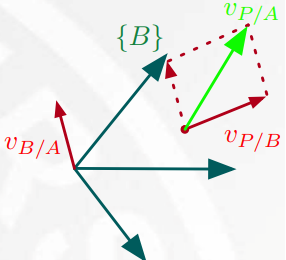
\includegraphics[width=.35\textwidth]{Linear Velocity}} \quad
\subfloat[旋转]{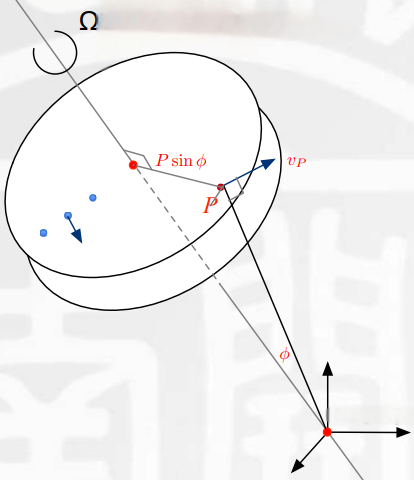
\includegraphics[width=.3\textwidth]{Rotational Motion}}
\caption[速度合成]{速度合成}
\end{figure}

\begin{itemize}
\item 相对速度:平行四边形法则,$ v_{P/A} = v_{B/A} + v_{P/B} $,$ v_{i/j} $指$ i $相对于$ j $坐标系的速度。
\item 旋转:垂直于原平面,$ v_p = \Omega \times P $,注意先后顺序。
\item 综合:$ ^A v_{P/A} = ^A v_{B/A} + ^A_B R \cdot ^B v_{P/B} + ^A \Omega \times (^A_B R \cdot ^B P) $,注意统一坐标系。
\end{itemize}
%------------------------------------------------
\paragraph{课程内容}
\begin{figure}[H]
\centering
\subfloat[控制系统]{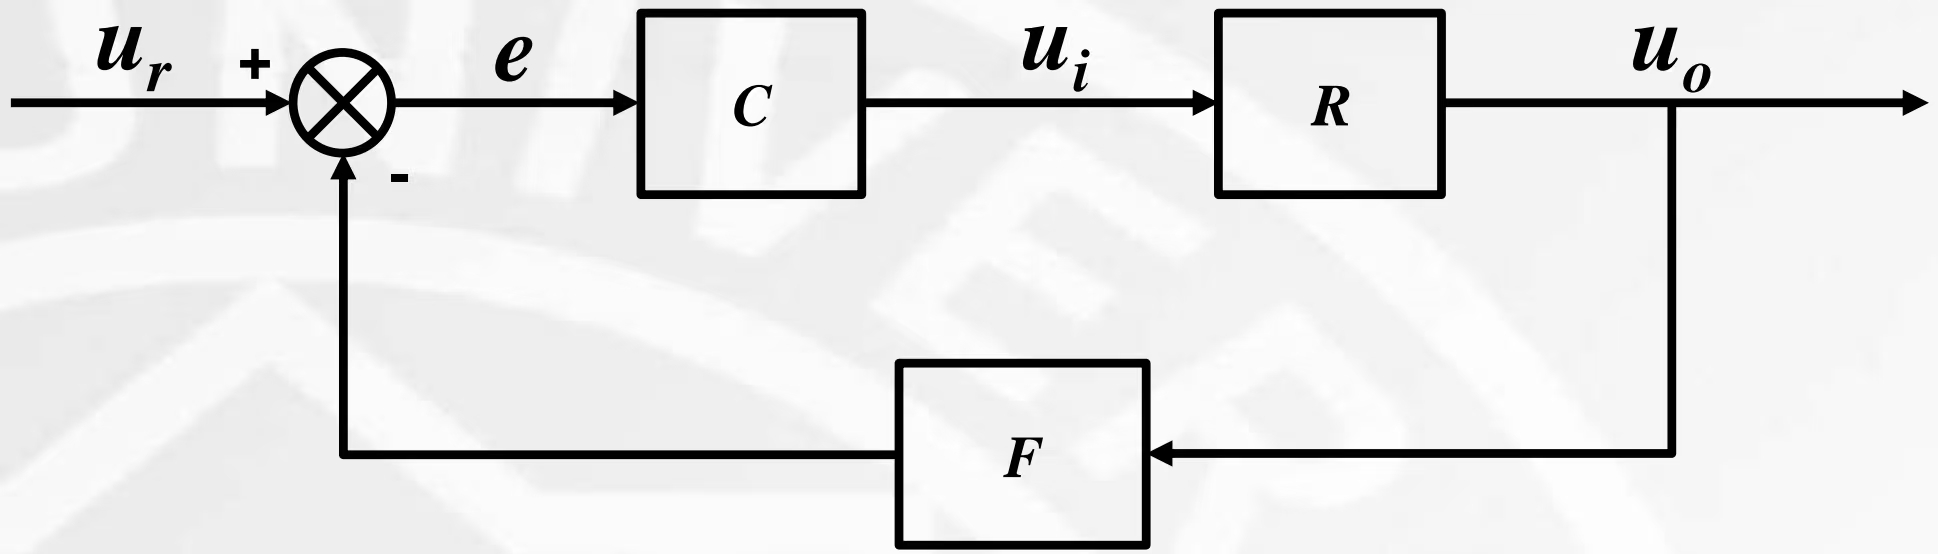
\includegraphics[width=.5\textwidth]{control}} \quad
\subfloat[正逆运动学]{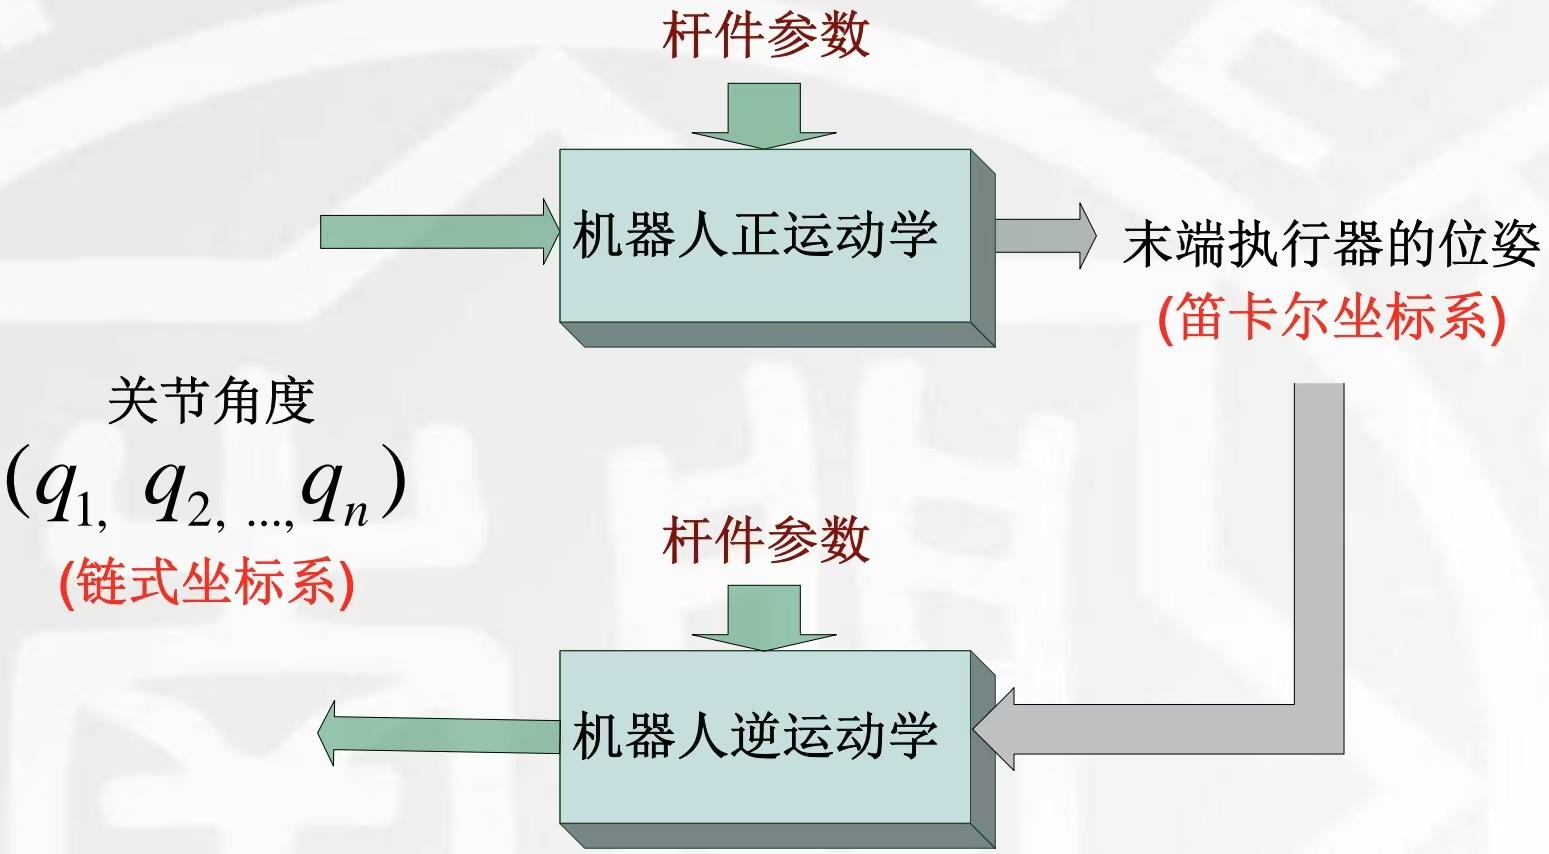
\includegraphics[width=.35\textwidth]{kinematics}}
\caption[课程内容]{课程内容}
\end{figure}

\begin{table}[hbt]
\caption{课程内容}
\centering
\begin{tabular}{|p{0.5cm}|p{2cm}|p{2cm}|p{2cm}|p{2cm}|p{2cm}|p{2cm}|p{2cm}|}
\hline
& $ u_i $ & $ u_o $ & $ R $ & $ F $ & $ u_r $ & $ e $ & $ C $ \\
\hline
概念 & 系统输入 & 系统输出 & 系统模型 & 反馈单元 & 系统给定 & 系统误差 & 控制器 \\
\hline
含义 & 能对被控对象施加作用的手段 & 作业目标相应的可测系统状态 & 系统输入输出映射 & 系统输出映射变换 & 系统作业目标 & 作业目标与系统当前测量状态差值 & 系统误差与输入映射 \\
\hline
内容 & \multicolumn{2}{c|}{空间描述与变换} & \multicolumn{2}{p{4cm}|}{正、逆运动学,雅可比,动力学} & 轨迹规划 & \multicolumn{2}{c|}{机器人控制} \\
\hline
\end{tabular}
\end{table}

\begin{itemize}
\item 正运动学($ f:q \rightarrow ^B E $):已知关节角度和位置,计算末端执行器位姿。
\item 逆运动学($ f:\{^B E\} \rightarrow q $):给定末端执行器位姿,求各关节需达到的角度和位置。
\end{itemize}
%----------------------------------------------------------------------------------------
\section{空间描述与变换}
%------------------------------------------------
\subsection[空间描述]{空间描述}
%------------------------------------------------
\subsubsection[坐标系]{坐标系}
\begin{itemize}
\item 笛卡尔坐标系$ (x, y, z) $:标准正交基,右手法则。
\item 圆柱坐标系$ (r, \theta, \mu) $:
$ \begin{cases}
x = r\cos\theta &r \geq 0 \\
y = r\sin\theta &0 \leq \theta \leq 2 \pi \\
z = \mu
\end{cases} $。
\item 球坐标系$ (r, \alpha, \beta) $:
$ \begin{cases}
x = r\cos\beta\cos\alpha &r \geq 0 \\
y = r\cos\beta\sin\alpha &0 \leq \alpha \leq 2\pi \\
z = r\sin\beta &0 \leq \beta \leq 2\pi
\end{cases} $。
\end{itemize}

\begin{figure}[H]
\centering
\subfloat[笛卡尔坐标系]{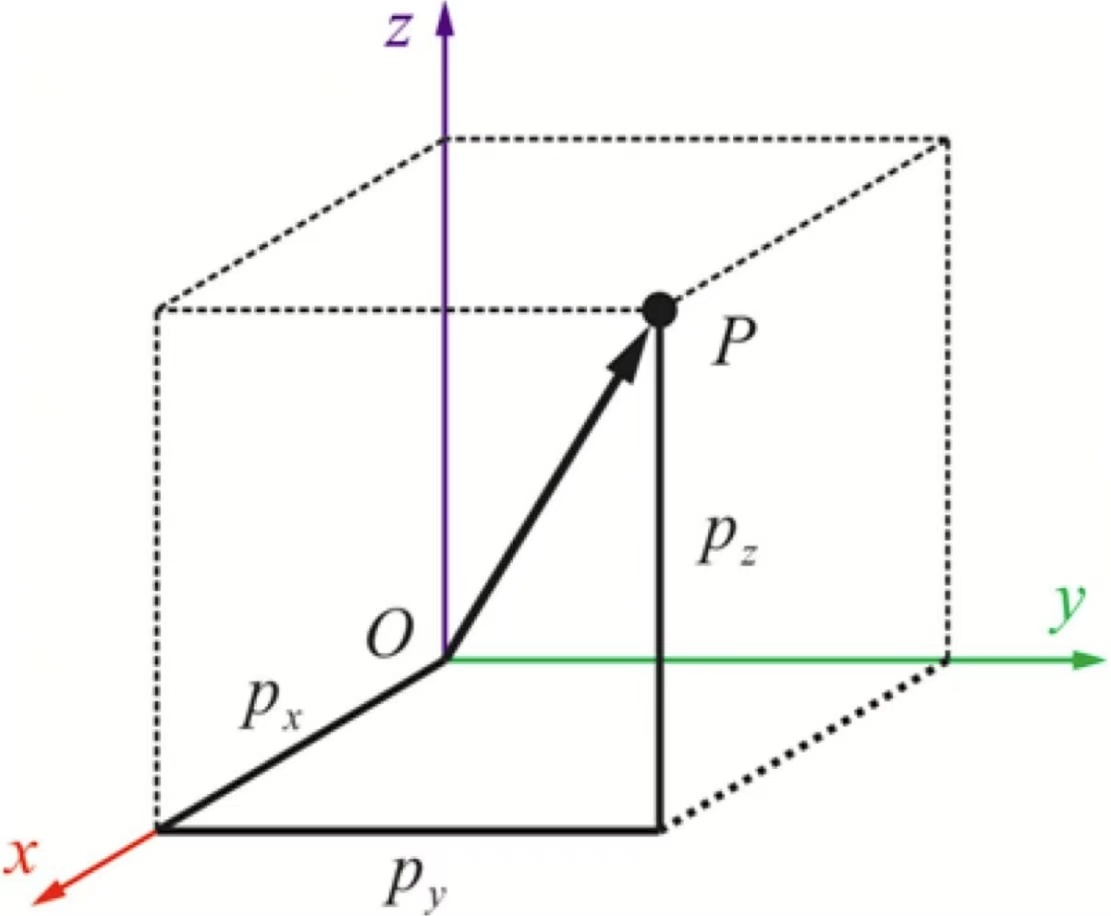
\includegraphics[width=.25\textwidth]{Cartesian}} \quad
\subfloat[圆柱坐标系]{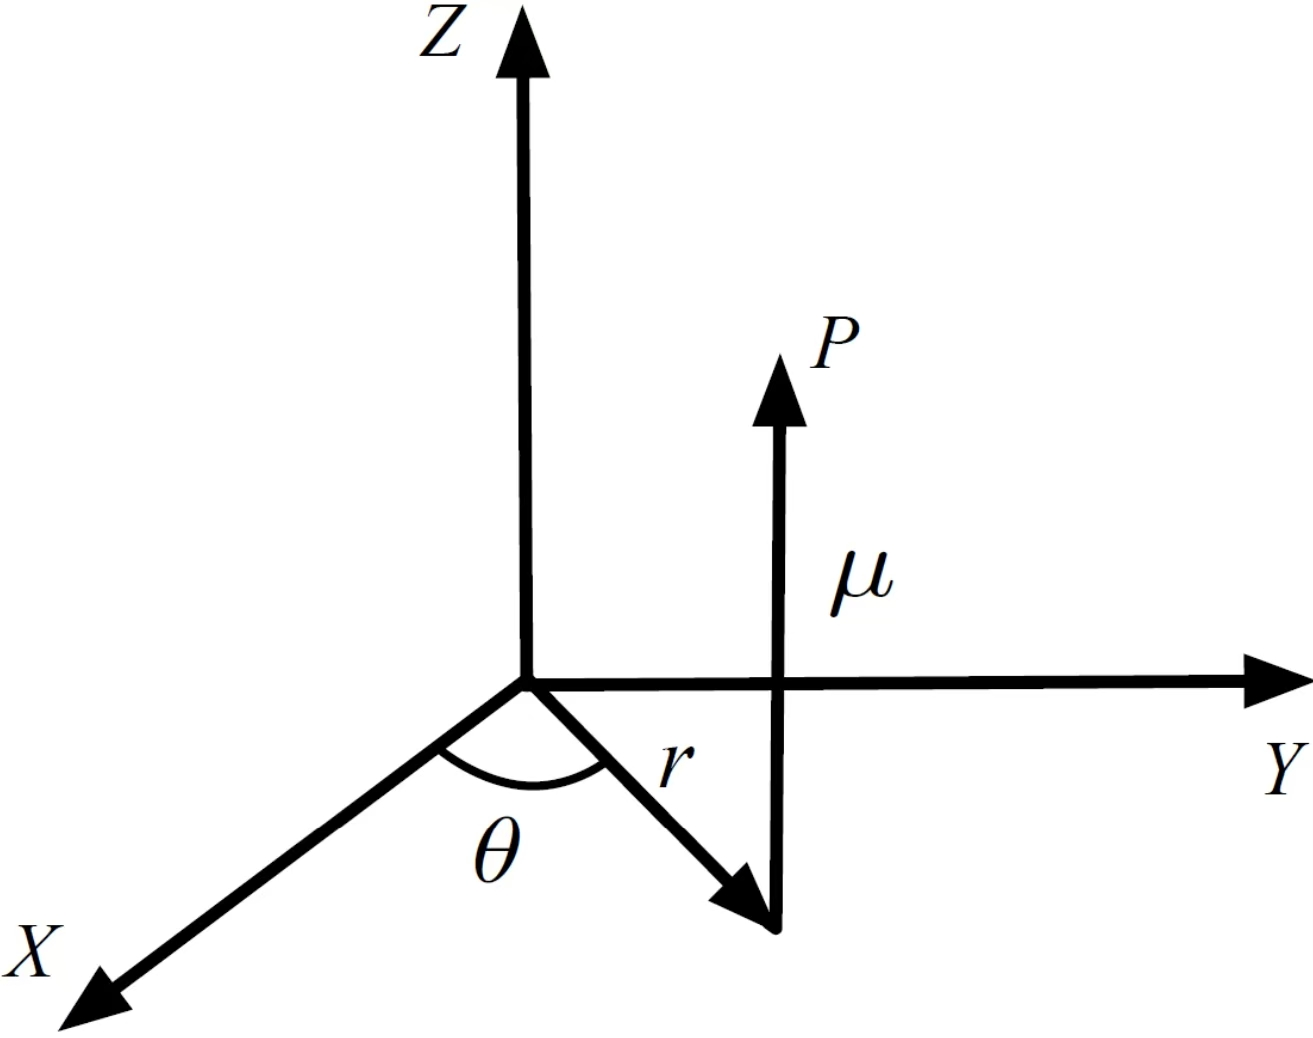
\includegraphics[width=.25\textwidth]{cylindrical}} \quad
\subfloat[球坐标系]{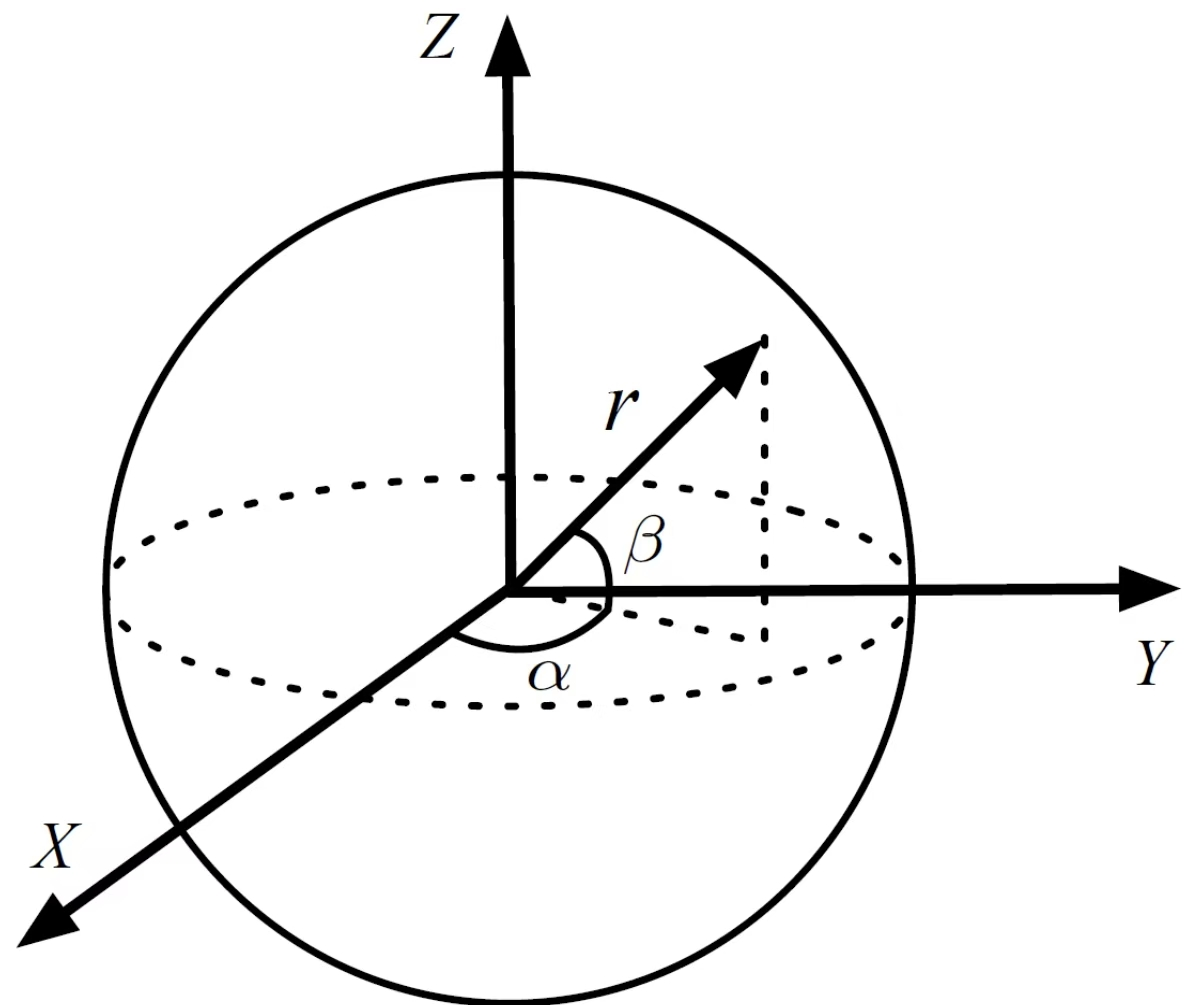
\includegraphics[width=.25\textwidth]{Spherical}}
\caption[坐标系]{坐标系}
\end{figure}
%------------------------------------------------
\subsubsection[刚体]{刚体}
\begin{itemize}
\item 刚体上任意两点间相对距离保持不变,角(加)速度相同。
\item 空间描述:位姿(Pose)=位置(Position)$ P_{Borg} $+姿态(Orientation)$ \{\vec x_B, \vec y_B, \vec z_B\} $。
\end{itemize}

\begin{figure}[H]
\centering 
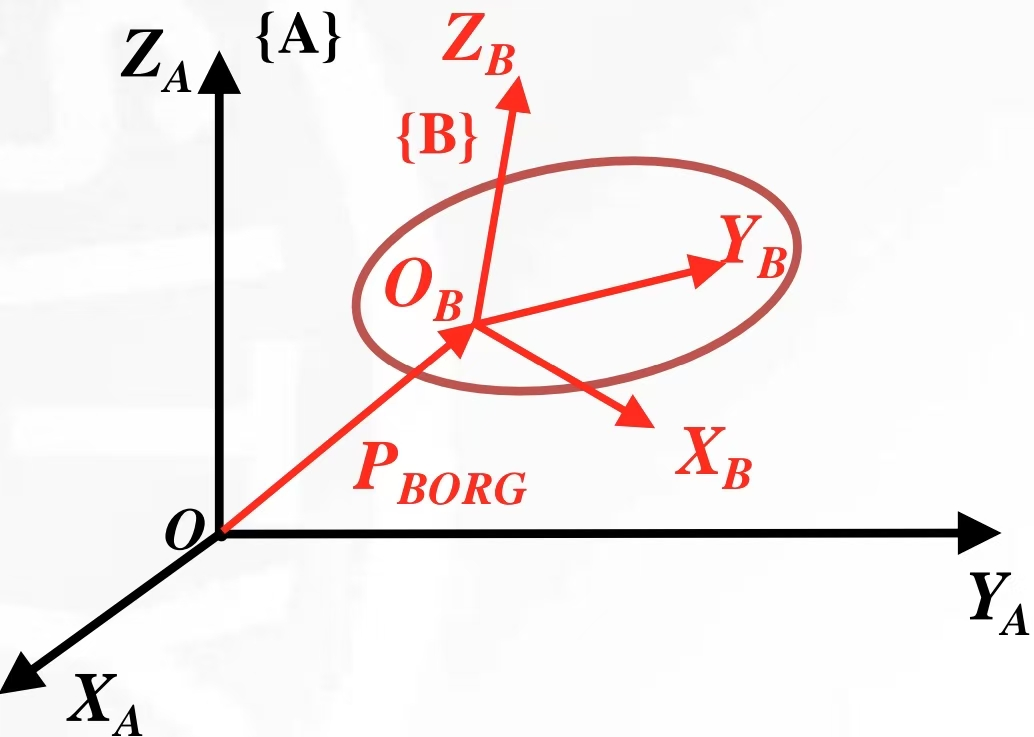
\includegraphics[width=0.3\textwidth]{rigid} 
\caption[刚体位姿]{刚体位姿}
\end{figure}
%------------------------------------------------
\subsection[变换]{变换}
%------------------------------------------------
\subsubsection[变换阵]{变换阵($ B \to A $)\tip{变换阵(逆变换)}}
%------------------------------------------------
\paragraph{旋转阵(Rotation Matrix)}
$ ^A X = ^A_B R \cdot ^B X $。
$$ 
^A_B R 
= \begin{bmatrix} r_{11} & r_{12} & r_{13} \\ r_{21} & r_{22} & r_{23} \\ r_{31} & r_{32} & r_{33} \end{bmatrix}
= \begin{bmatrix} ^A \vec x_B & ^A \vec y_B & ^A \vec z_B \end{bmatrix}
= \begin{bmatrix} ^B \vec x_A^T \\ ^B \vec y_A^T \\ ^B \vec z_A^T \end{bmatrix}
= \begin{bmatrix} X_BX_A & Y_BX_A & Z_BX_A \\ X_BY_A & Y_BY_A & Z_BY_A \\ X_BZ_A & Y_BZ_A & Z_BZ_A \end{bmatrix}
\in R^{3 \times 3}
$$
\begin{itemize}
\item 单位正交阵$ ^A_B R $满秩。
\item 求解:每列是B的基在A下的表示,每行是A的基在B下的表示。
\item $ ^A_B R^{-1} = ^A_B R^T = ^B_A R $。
\end{itemize}
%------------------------------------------------
\paragraph{齐次变换阵}
$ ^A_B T = \begin{bmatrix} ^A_B R & ^A P_{Borg} \\ 0 & 1 \end{bmatrix} $。
\begin{itemize}
\item $ ^A_B T $满秩。其中右下角的$ 1 $是比例,左下角的$ 0 $是透视变换。
\item 求解:求$ ^A_B R $,填底行,求$ P_{Borg} $(沿$ A $坐标系,即旋转完的$ B $坐标系,$ B $到$ A $的移动)。
\item 
$ 
^A_B T^{-1} = ^B_A T 
= \begin{bmatrix} ^B_A R & ^B P_{Aorg} \\ \mathbf{0} & 1 \end{bmatrix} 
= \begin{bmatrix} ^A_B R^T & -^A_B R^T \cdot ^A P_{Borg} \\ \mathbf{0} & 1 \end{bmatrix} 
$,

推导:$ ^B(^A P_{Borg}) = ^B_A R \cdot ^A P_{Borg} + ^B P_{Aorg} = 0 $。
\end{itemize}
%------------------------------------------------
\subsubsection[坐标系映射]{坐标系映射(Mapping)——不同坐标系,右乘}
$ ^A P = ^A_B R \cdot ^B P + ^A P_{Borg} = ^A_B T \cdot ^B P $。
\begin{itemize}
\item 由$ B $到$ A $。
\item 旋转映射:$ ^A P = ^A_B R \cdot ^B P $。 \\
平移映射:同一个点不同向量。$ ^A P = ^A P_{Borg} + ^B P $。
\item 分开计算旋转和平移时,一般先旋转后平移(不同坐标系的矢量只有在坐标系姿态相同时才可以加减)。
\end{itemize}
%------------------------------------------------
\subsubsection[向量变换算子]{向量变换算子(Operator)——同一坐标系,左乘}
$ ^A P_2 = R_K(\theta) \cdot ^A P_1 + ^A Q= T \cdot ^A P_1 $。
\begin{itemize}
\item 由$ P_1 $到$ P_2 $。
\item 旋转算子(绕$ k $转$ \theta $角,右手系正方向)\tip{旋转算子}:$ ^A P_2 = R_K(\theta) \cdot ^AP_1 $。 \\
$$
R_x(\theta) = \begin{bmatrix} 1 & 0 & 0 \\ 0 & \cos\theta & -\sin\theta \\ 0 & \sin\theta & \cos\theta \end{bmatrix}, 
R_y(\theta) = \begin{bmatrix} \cos\theta & 0 & \sin\theta \\ 0 & 1 & 0 \\ -\sin\theta & 0 & \cos\theta \end{bmatrix}, 
R_z(\theta) = \begin{bmatrix} \cos\theta & -\sin\theta & 0 \\ \sin\theta & \cos\theta & 0 \\ 0 & 0 & 1 \end{bmatrix}
$$ \\
平移算子:两个点两个向量。$ ^A P_2 = \begin{bmatrix} E & q \\ 0 & 1 \end{bmatrix} + ^A P_1 $。
\end{itemize}
%------------------------------------------------
\subsubsection[对比]{对比\tip{映射与算子}}
\begin{minipage}{0.58\textwidth}
\begin{figure}[H]
\centering
\subfloat[旋转映射(不同坐标系)]{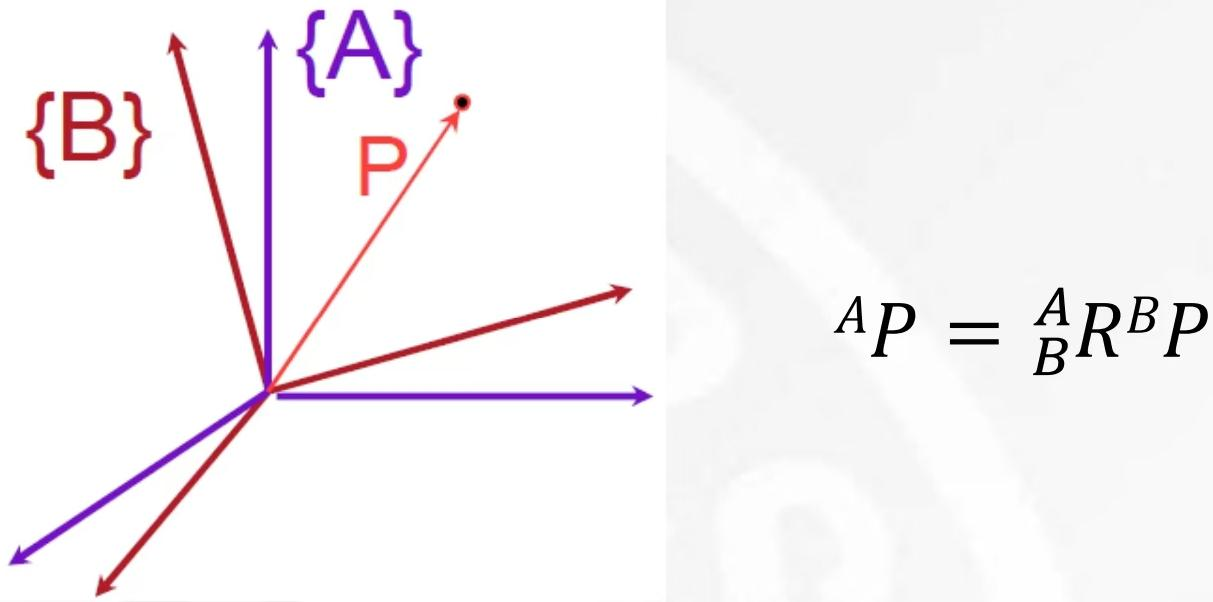
\includegraphics[width=.45\textwidth]{Mapping_r}} \quad
\subfloat[旋转算子(同一坐标系)]{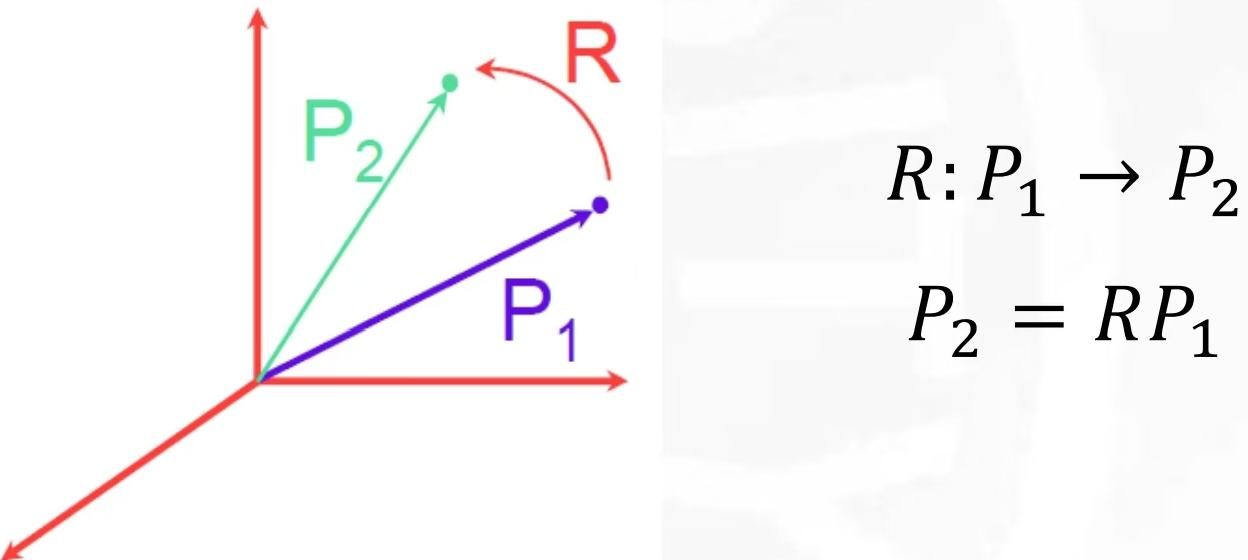
\includegraphics[width=.45\textwidth]{Operator_r}}\\
\subfloat[平移映射(不同坐标系)]{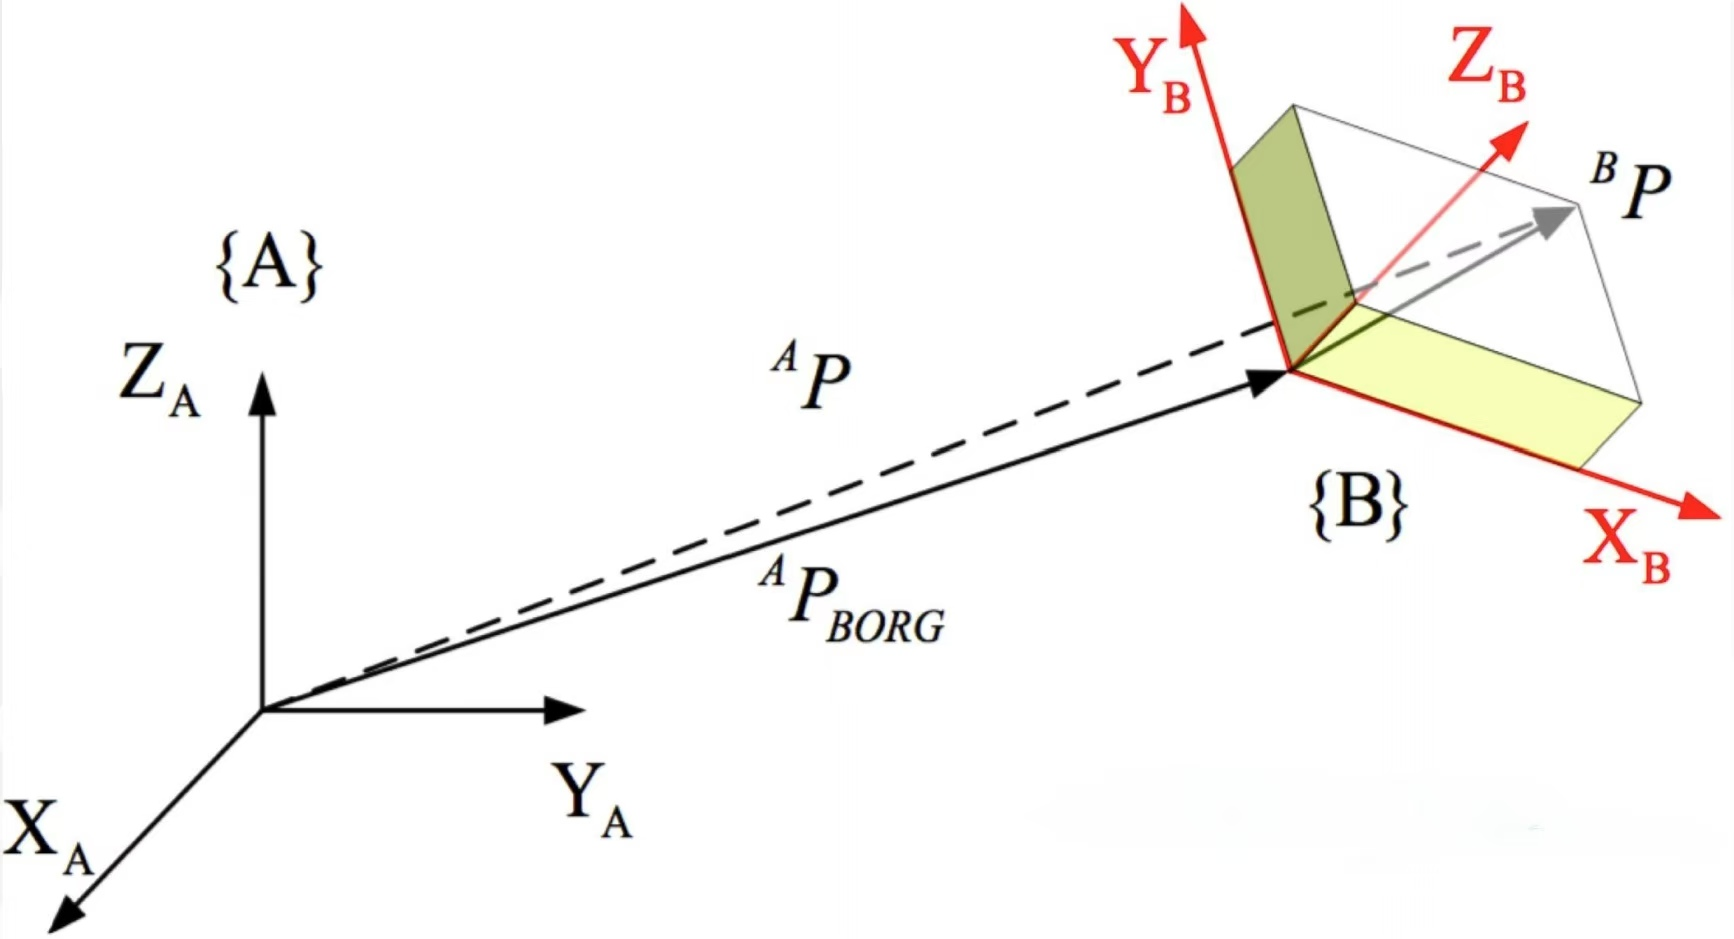
\includegraphics[width=.45\textwidth]{Mapping_p}} \quad
\subfloat[平移算子(同一坐标系)]{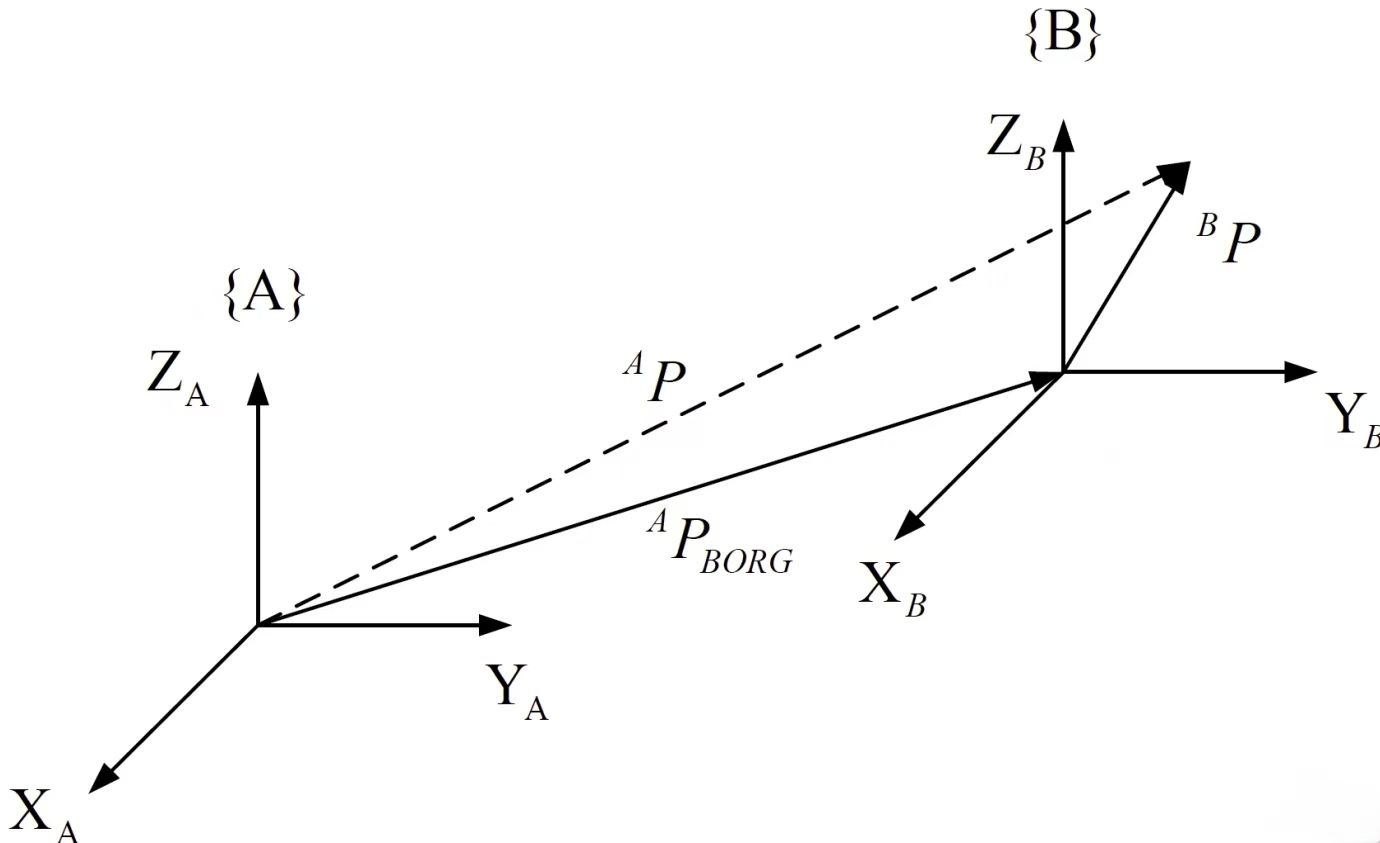
\includegraphics[width=.45\textwidth]{Operator_p}}
\caption[映射与算子对比]{映射与算子对比}
\end{figure}
\end{minipage}
\hfill
\begin{minipage}{0.38\textwidth}
\centering
\captionof{table}{映射与算子对比}
\begin{tabular}{c|cc}
\hline
& 映射 & 算子 \\
\hline
坐标系 & 不同 & 同一 \\
连乘 & 右乘 & 左乘 \\
\hline
\end{tabular}
\end{minipage}
%------------------------------------------------
\subsubsection[复合变换]{复合变换\tip{复合变换}}
\begin{itemize}
\item $ ^A_C T = ^A_B T \cdot ^B_C T $:左下消右上,链式。
\item 计算顺序与计算量:$ ^A P = ^A_B T \cdot ^B_C T \cdot ^C P $从左向右先推导旋转阵比从右向左依次变换计算量大很多。
\end{itemize}
%------------------------------------------------
\subsection[姿态描述]{姿态描述}
%------------------------------------------------
\subsubsection[描述方式]{描述方式}
%------------------------------------------------
\paragraph{旋转矩阵与方向余弦}
\begin{itemize}
\item 旋转矩阵$ R = \begin{bmatrix} r_{11} & r_{12} & r_{13} \\ r_{21} & r_{22} & r_{23} \\ r_{31} & r_{32} & r_{33} \end{bmatrix} $
$ \Leftrightarrow $
方向余弦$ x_r = \begin{bmatrix} {r_1}_{(3 \times 1)} \\ {r_2}_{(3 \times 1)} \\ {r_3}_{(3 \times 1)} \end{bmatrix}_{(9 \times 1)} $。
\item $ 9 $个变量,$ 6 $个约束(单位+正交),$ 3 $个独立变量。
\end{itemize}
%------------------------------------------------
\paragraph{等效轴角(绕空间中一轴旋转)}\tip{等效轴角}
\begin{itemize}
\item 目标:坐标轴$ B $绕$ ^A \hat{k} = \begin{bmatrix} k_x & k_y & k_z \end{bmatrix}^T(k_x^2 + k_y^2 + k_z^2 = 1) $旋转$ \theta $角。
\item 方法:先使坐标轴$ B $与坐标轴$ A $重合,再使一轴(以下以$ z $轴为例)与$ ^A \hat{k} $重合,最后绕重合轴旋转$ \theta $角。
\item 
\begin{align*}
R(\theta, ^A \hat{k}) &= R_K(\theta) = R_z(\alpha) \cdot R_y(\beta) \cdot R_z(\theta) \cdot R_y^T(\beta) \cdot R_z^T(\alpha) \\
&= \begin{bmatrix}
k_x k_x v\theta + c\theta & k_x k_y v\theta - k_z s\theta & k_x k_z v\theta + k_y c\theta \\
k_x k_y v\theta + k_z s\theta & k_y k_y v\theta + c\theta & k_y k_z v\theta - k_x s\theta \\
k_x k_z v\theta - k_y c\theta & k_y k_z v\theta + k_x s\theta & k_z k_z v\theta + c\theta
\end{bmatrix} 
\end{align*}

其中$ c\theta = \cos\theta, s\theta = \sin\theta, v\theta = 1 - \cos\theta $。
\item 与旋转矩阵结合:
$$ \theta = \arccos(\frac{r_{11} + r_{22} + r_{33} - 1}{2}) $$
$$ ^A \hat{k} = \frac{1}{2 \sin θ} \begin{bmatrix} r_{32} - r_{23} & r_{13} - r_{31} & r_{21} - r_{12} \end{bmatrix}^T $$
\begin{itemize}
\item 奇异:$ \sin\theta = 0 $。
\item 多解:$ \arccos $多解。
\end{itemize}
\end{itemize}
%------------------------------------------------
\paragraph{四元数(欧拉参数)}\tip{四元数}~\\

由轴$ \hat{k} = \begin{bmatrix} k_x & k_y & k_z \end{bmatrix}^T(k_x^2 + k_y^2 + k_z^2 = 1) $和$ \theta $,
得到欧拉参数:$$ \varepsilon_1 = k_x \sin\frac{\theta}{2}, \varepsilon_2 = k_y \sin\frac{\theta}{2}, \varepsilon_3 = k_z \sin\frac{\theta}{2}, \varepsilon_4 = \cos\frac{\theta}{2} $$

有$ \varepsilon_1^2 + \varepsilon_2^2 + \varepsilon_3^2 + \varepsilon_4^2 = 1 $,
其表示超球体上一点,至少有一个参数不小于$ \frac{1}{2} $。

表示为旋转阵
$ 
R =
\begin{bmatrix}
1 - 2(\varepsilon_2^2 + \varepsilon_3^2) & 2(\varepsilon_1 \varepsilon_2 - \varepsilon_3 \varepsilon_4) & 2(\varepsilon_1 \varepsilon_3 + \varepsilon_2 \varepsilon_4) \\
2(\varepsilon_1 \varepsilon_2 + \varepsilon_3 \varepsilon_4) & 1 - 2(\varepsilon_1^2 + \varepsilon_3^2) & 2(\varepsilon_2 \varepsilon_3 - \varepsilon_1 \varepsilon_4) \\
2(\varepsilon_1 \varepsilon_3 - \varepsilon_2 \varepsilon_4) & 2(\varepsilon_2 \varepsilon_3 + \varepsilon_1 \varepsilon_4) & 1 - 2(\varepsilon_1^2 + \varepsilon_2^2)
\end{bmatrix} 
$

求解时,先计算最大的$ \varepsilon_i $,用其计算其它参数,以保证最高精度。以下以$ \varepsilon_4 $为例:
\begin{itemize}
\item $ tr(R) = r_{11} + r_{22} + r_{33} = 3 - 4(\varepsilon_1^2 + \varepsilon_2^2 + \varepsilon_3^2) = 3 - 4(1 - \varepsilon_4^2) $。
\item $ \varepsilon_4 = \frac{1}{2} \sqrt{1 + r_{11} + r_{22} + r_{33}} $。
\item $ \varepsilon_1 = \frac{r_{32} - r_{23}}{4 \varepsilon_4}, \varepsilon_2 = \frac{r_{13} - r_{31}}{4 \varepsilon_4}, \varepsilon_3 = \frac{r_{21} - r_{12}}{4 \varepsilon_4} $。
\end{itemize}
%------------------------------------------------
\subsubsection[旋转角]{旋转角}
\begin{itemize}
\item 固定角(12种):绕同一坐标轴旋转,算子左乘。
\item 变角(12种):绕变换坐标轴旋转,映射右乘。
\begin{itemize}
\item 泰特布莱恩角:三个旋转轴不同,$ Z-Y-X $泰特布莱恩角与$ X-Y-Z $固定角对偶。
\item 欧拉角:第一个旋转轴与最后一个旋转轴相同,奇异现象(中间旋转导致前后旋转轴重合,自由度丢失)。
\end{itemize}
\end{itemize}
%----------------------------------------------------------------------------------------
\section{正运动学}
%------------------------------------------------
\subsection[机器人结构与自由度]{机器人结构与自由度}
%------------------------------------------------
\paragraph{自由刚体空间运动}
6个自由度,沿$ x,y,z $轴的平移和旋转。
%------------------------------------------------
\paragraph{运动副与约束}
运动副(Kinematic pairs)为构件间连接结构,使构件只能相对运动(受约束),自由度减少。
\begin{itemize}
\item 低副:面接触,压强低。如旋转副、平移副。 \\
高副:点/线接触,压强高,易磨损。如凸轮副、齿轮副。
\item 根据引入的约束数目分类。
\item 转动副和移动副。
\end{itemize}
%------------------------------------------------
\paragraph{关节与连杆}
\begin{itemize}
\item 关节(Joint):连接各构件的、能主动驱动产生相对运动的运动副,一个关节提供$ 5 $个约束,只有$ 1 $个自由度。
\begin{itemize}
\item 转动关节(Revolute joint)
\item 移动关节(Prismatic joint)
\end{itemize}
\item 连杆(Link):组成机器人的、由关节连接形成运动链的刚体,传递运动和力,一个自由连杆提供$ 6 $个自由度。
\begin{itemize}
\item 固定连杆(基座)
\item 运动连杆
\end{itemize}
\item 自由度=运动连杆数=关节数。
\item 冗余机器人:自由度大于$ 6 $的空间机器人和自由度大于$ 3 $的平面机器人。
可以增加灵活性,避免奇异,提升避障能力,但因为逆运动学多解而求解复杂。
\end{itemize}
%------------------------------------------------
\subsection[DH参数]{DH参数}
%------------------------------------------------
\subsubsection[定义]{定义}
\begin{figure}[H]
\centering 
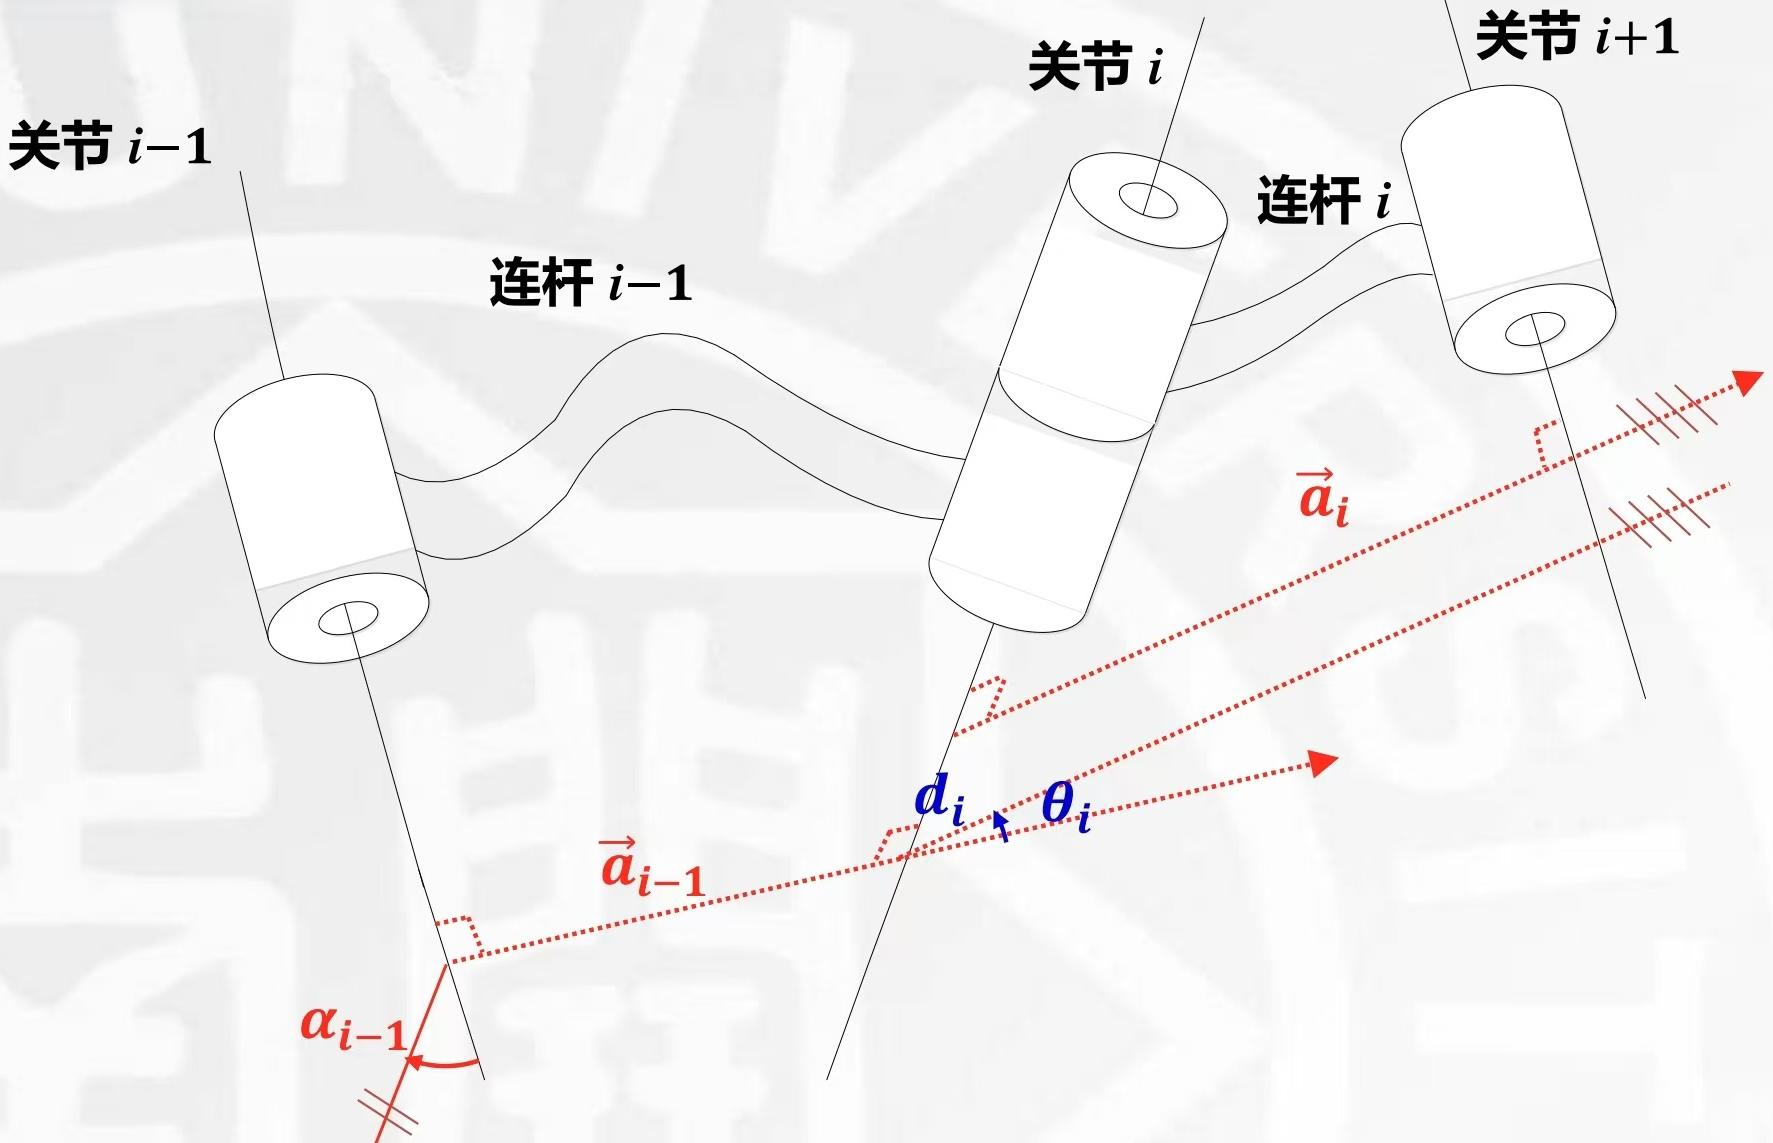
\includegraphics[width=0.5\textwidth]{dh} 
\caption[DH参数]{DH参数定义}
\end{figure}

对于关节$ i $:
\begin{itemize}
\item 连杆参数(几何参数):沿$ X_{i - 1} $,由$ Z_{i - 1} $与$ Z_i $求取,定值。
\begin{itemize}
\item 连杆长度(Link Length)$ \vec a_{i - 1}  $:公垂线段(除平行外唯一)长度。
\item 连杆扭角(Link Twist)$ \alpha_{i - 1} $:右手法则(指向末端)。
\end{itemize}
\item 关节参数(运动参数):沿$ Z_i $,由$ X_{i - 1} $与$ X_i $求取,
平移关节$ \theta_i $为定值,旋转关节$ d_i $为定值,另一个为变量。
\begin{itemize}
\item 关节偏距(Joint Offset)$ d_i $:公垂线间距离。
\item 关节转角(Joint Angle)$ \theta_i $:公垂线夹角。
\end{itemize}
\item 基座:虚拟关节$ 0 $与关节$ 1 $重合,$ \vec a_0 = 0, \alpha_0 = 0 $。 \\
末端:虚拟关节$ n + 1 $与关节$ n $重合,$ \vec a_n = 0, \alpha_n = 0 $。
\item 关节$ i $的DH参数表征其所在坐标系与前一坐标系的关系。 \\
坐标系$ i $的参数表征连杆$ i $沿其$ z $轴运动后相对于连杆$ i - 1 $的位姿。
\end{itemize}

\begin{minipage}{0.48\textwidth}
\centering
\captionof{table}{DH参数表}
\begin{tabular}{c|cccc}
\hline
关节 & $ \alpha_{i - 1} $ & $ \vec a_{i - 1} $ & $ \theta_i $ & $ d_i $ \\
\hline
1 & $ 0 $ & $ 0 $ & $ \theta_1 $ & $ d_1 $ \\
2 & $ \alpha_1 $ & $ \vec a_1 $ & $ \theta_2 $ & $ d_2 $ \\
\hline
\end{tabular}
\end{minipage}
\hfill
\begin{minipage}{0.48\textwidth}
\centering
\captionof{table}{DH参数情况讨论}
\begin{tabular}{c|cc}
\hline
相邻轴关系 & 角 & 距离 \\
\hline
共线 & $ 0 $ & $ 0 $ \\
平行 & $ 0 $ & $ d $ \\
相交 & $ \theta $ & $ 0 $ \\
不相交 & $ \theta $ & $ d $ \\
\hline
\end{tabular}
\end{minipage}
%------------------------------------------------
\subsubsection[求解]{求解\tip{DH参数求解}}
\begin{enumerate}
\item $ Z_i $轴:关节$ i $轴延长线,标注正方向。
\item $ X_i $轴:$ Z_{i - 1} $轴与$ Z_i $轴公垂线(由前者指向后者)或交点(垂直平面,一般指向末端)。
\item ($ Y_i $轴:$ Z_i $轴与$ X_i $轴公垂线,右手法则确定。)
\item 标注基座坐标系和末端坐标系,尽可能与相邻坐标系重合。
\item 制表,并根据关节的平移或旋转属性在对应位置标注变量。
\item 沿$ X_{i - 1} $,由$ Z_{i - 1} $与$ Z_i $求取$ \vec a_{i - 1}  $和$ \alpha_{i - 1} $。
\item 沿$ Z_i $,由$ X_{i - 1} $与$ X_i $求取$ d_i $和$ \theta_i $。
\end{enumerate}
%------------------------------------------------
\paragraph{例题}
\begin{figure}[H]
\centering
\subfloat[例1结构图]{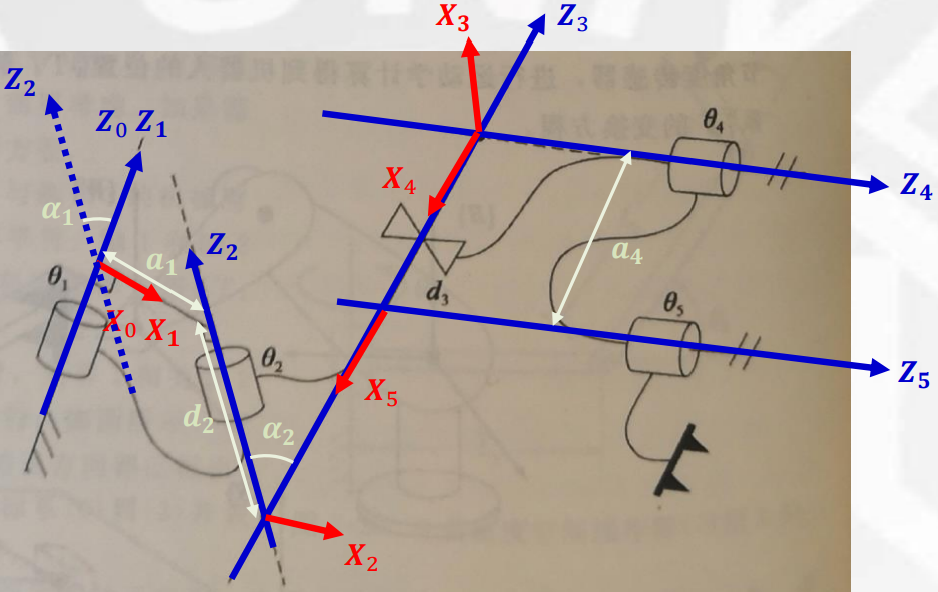
\includegraphics[width=.3\textwidth]{1.1.1}} \quad
\subfloat[例2结构图]{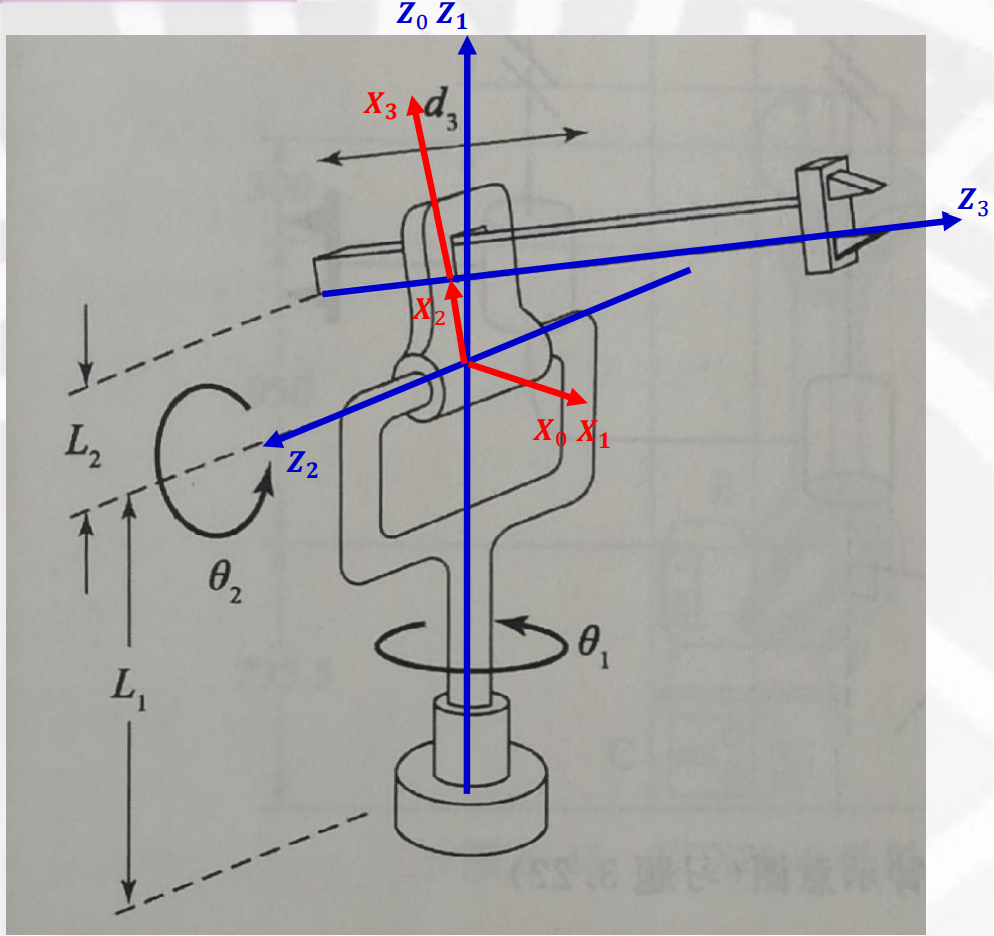
\includegraphics[width=.3\textwidth]{1.2.1}} \\
\subfloat[例1参数表]{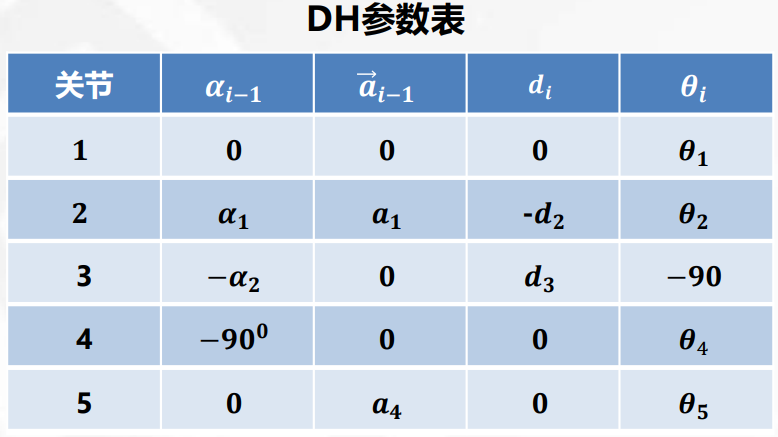
\includegraphics[width=.3\textwidth]{1.1.2}} \quad
\subfloat[例2参数表]{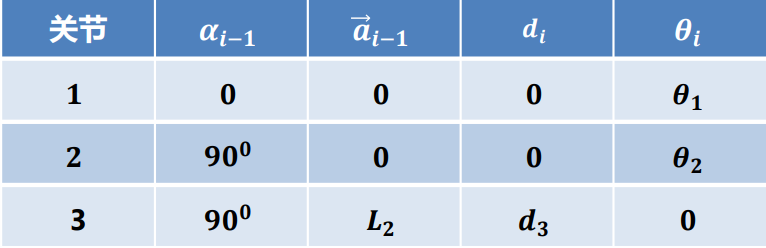
\includegraphics[width=.3\textwidth]{1.2.2}} \\
\subfloat[例3结构图]{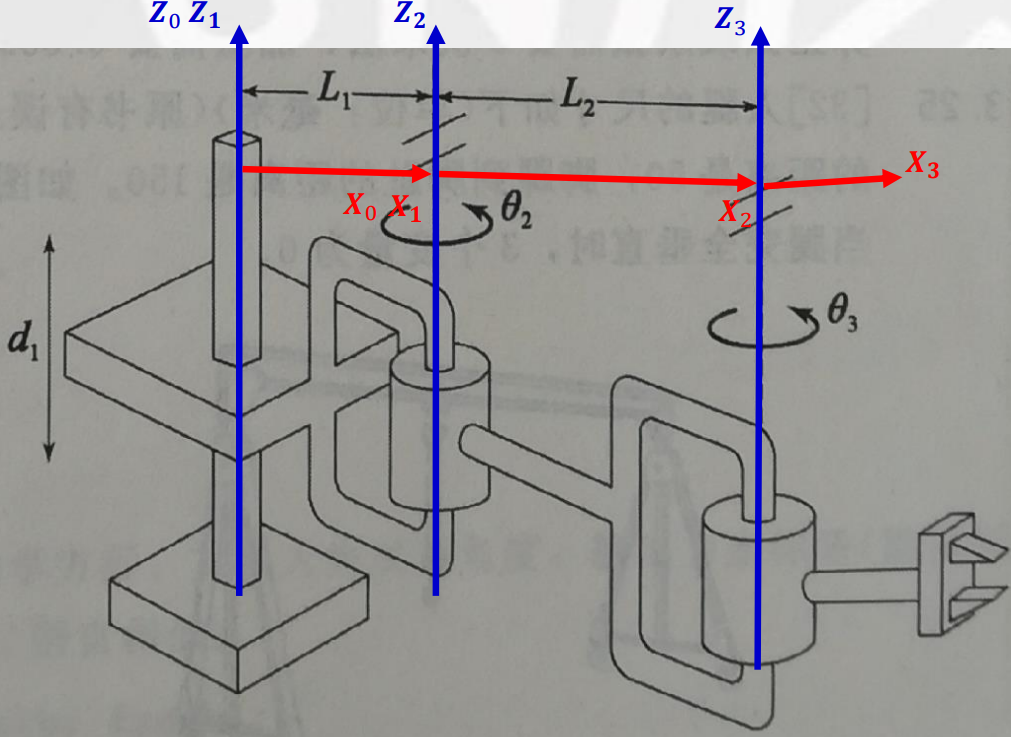
\includegraphics[width=.3\textwidth]{1.3.1}} \quad
\subfloat[例4结构图]{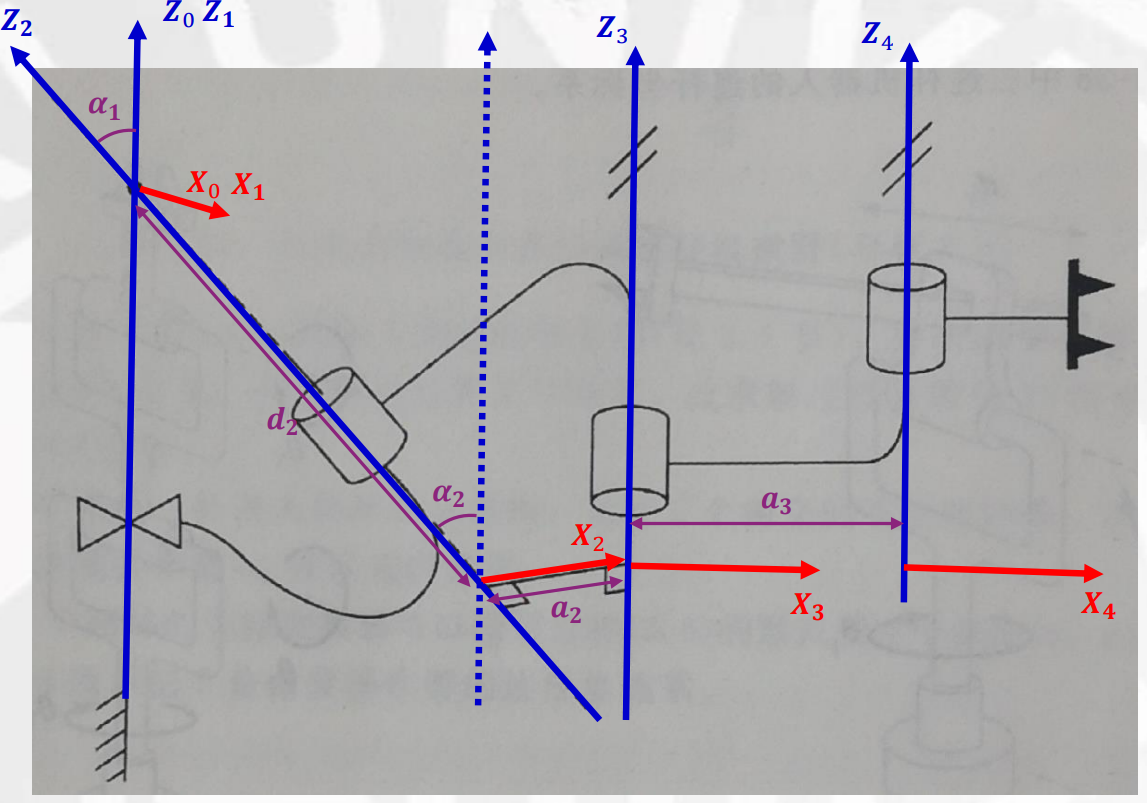
\includegraphics[width=.3\textwidth]{1.4.1}} \\
\subfloat[例3参数表]{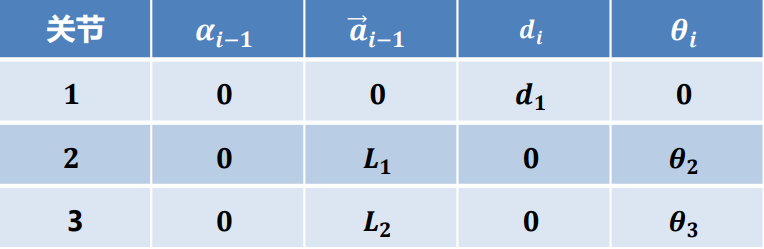
\includegraphics[width=.3\textwidth]{1.3.2}} \quad
\subfloat[例4参数表]{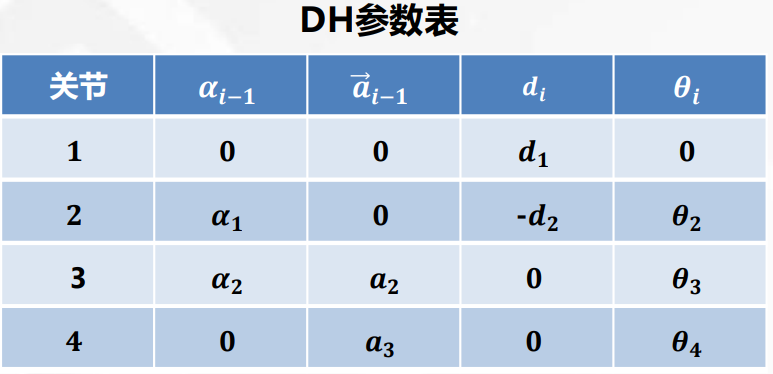
\includegraphics[width=.3\textwidth]{1.4.2}}
\caption[DH参数例题]{DH参数例题}
\end{figure}
%------------------------------------------------
\subsection[正运动学方程]{正运动学方程\tip{正运动学方程}}
先根据连杆参数沿$ X $轴变换,再根据关节参数沿新$ Z $轴变换:
\begin{align*}
^{i - 1}_i T 
&= 
\begin{bmatrix} 1 & 0 & 0 & \vec a_{i - 1} \\ 0 & \cos \alpha_{i - 1} & -\sin \alpha_{i - 1} & 0 \\ 0 & \sin \alpha_{i - 1} & \cos \alpha_{i - 1} & 0 \\ 0 & 0 & 0 & 1 \end{bmatrix}
\begin{bmatrix} \cos \theta_i & -\sin \theta_i & 0 & 0 \\ \sin \theta_i & \cos \theta_i & 0 & 0 \\ 0 & 0 & 1 & d_i \\ 0 & 0 & 0 & 1 \end{bmatrix} \\
&= 
\begin{bmatrix} \cos\theta_i & -\sin\theta_i & 0 & \vec a_{i-1} \\ \sin\theta_i\cos\alpha_{i-1} & \cos\theta_i\cos\alpha_{i-1} & -\sin\alpha_{i-1} & -d_i\sin\alpha_{i-1} \\ \sin\theta_i\sin\alpha_{i-1} & \cos\theta_i\sin\alpha_{i-1} & \cos\alpha_{i-1} & d_i\cos\alpha_{i-1} \\ 0 & 0 & 0 & 1 \end{bmatrix}
\end{align*}

\begin{itemize}
\item 没有关于$ Y $轴的运动,静态的。
\item 按关节逐次变换,最终得到腕部坐标,而非末端坐标。
\end{itemize} 
%------------------------------------------------
\paragraph{例题}\label{sec:example2.1}~\\
\begin{minipage}{0.48\textwidth}
\centering
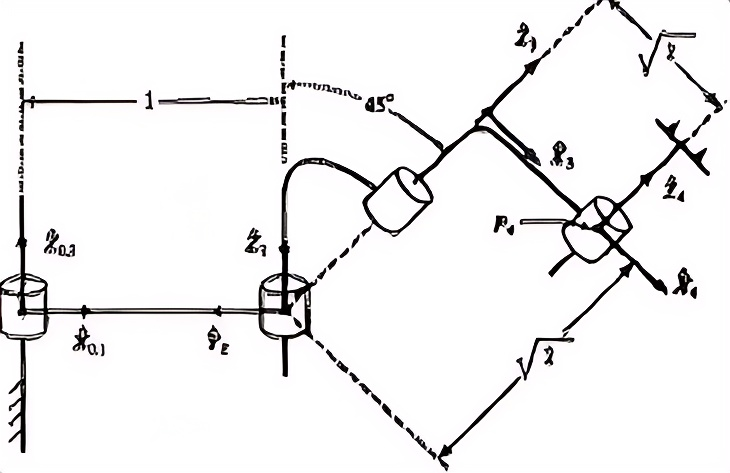
\includegraphics[width=0.95\textwidth]{2.1}
\captionof{figure}{正运动学方程例题}
\end{minipage}
\hfill
\begin{minipage}{0.48\textwidth}
\centering
\captionof{table}{正运动学方程例题DH参数表}
\begin{tabular}{c|cccc}
\hline
$ i $ & $ \alpha_{i - 1} $ & $ a_{i - 1} $ & $ \theta_i $ & $ d_i $ \\
\hline
1 & $ 0 $ & $ 0 $ & $ \theta_1 $ & $ 0 $ \\
2 & $ 0 $ & $ 1 $ & $ \theta_2 $ & $ 0 $ \\
3 & $ \frac{\pi}{4} $ & $ 1 $ & $ \theta_3 $ & $ 0 $ \\
4 & $ 0 $ & $ \sqrt{2} $ & $ \theta_4 $ & $ 0 $ \\
\hline
\end{tabular}
\end{minipage}
{\footnotesize
由其转化得到各齐次阵:
$$
^0_1T = \begin{bmatrix} c_1 & -s_1 & 0 & 0 \\ s_1 & c_1 & 0 & 0 \\ 0 & 0 & 1 & 0 \\ 0 & 0 & 0 & 1 \end{bmatrix},
^1_2T = \begin{bmatrix} c_2 & -s_2 & 0 & 1 \\ s_2 & c_2 & 0 & 0 \\ 0 & 0 & 1 & 0 \\ 0 & 0 & 0 & 1 \end{bmatrix},
^2_3T = \begin{bmatrix} c_3 & -s_3 & 0 & 0 \\ \frac{\sqrt{2}}{2}s_3 & \frac{\sqrt{2}}{2}c_3 & \frac{\sqrt{2}}{2} & 1 \\ -\frac{\sqrt{2}}{2}s_3 & -\frac{\sqrt{2}}{2}c_3 & \frac{\sqrt{2}}{2} & 1 \\ 0 & 0 & 0 & 1 \end{bmatrix},
^3_4T = \begin{bmatrix} c_4 & -s_4 & 0 & \sqrt{2} \\ s_4 & c_4 & 0 & 0 \\ 0 & 0 & 1 & 0 \\ 0 & 0 & 0 & 1 \end{bmatrix}
$$

最终得到正运动学方程:
$$
^0_4T = 
\begin{bmatrix}
c_{12}c_{34} - \frac{\sqrt{2}}{2}s_{12}s_{34} & -c_{12}s_{34} - \frac{\sqrt{2}}{2}s_{12}c_{34} & -\frac{\sqrt{2}}{2}s_{12} & c_1 + s_{12} + \sqrt{2}c_{12}c_3 - s_{12}s_3 \\
s_{12}c_{34} + \frac{\sqrt{2}}{2}c_{12}s_{34} & -s_{12}s_{34} + \frac{\sqrt{2}}{2}c_{12}c_{34} & \frac{\sqrt{2}}{2}c_{12} & s_1 - c_{12} + \sqrt{2}s_{12}c_3 + c_{12}s_3 \\
\frac{\sqrt{2}}{2}s_{34} & \frac{\sqrt{2}}{2}c_{34} & \frac{\sqrt{2}}{2} & s_3 + 1 \\
0 & 0 & 0 & 1
\end{bmatrix}
$$

续\ref{sec:example2.2},逆运动学求解。
}
%----------------------------------------------------------------------------------------
\section{逆运动学}
%------------------------------------------------
\subsection[逆运动学求解]{逆运动学求解\tip{逆运动学求解}}
由$ T = \begin{bmatrix} r_{11} & r_{12} & r_{13} & p_x \\ r_{21} & r_{22} & r_{23} & p_y \\ r_{31} & r_{32} & r_{33} & p_z \\ 0 & 0 & 0 & 1 \end{bmatrix} $
求解关节角度。
%------------------------------------------------
\subsubsection[方法]{方法}
\begin{itemize}
\item 代数法:利用平方($ \sin^2x + \cos^2x = 1 $)、和差角公式等化简齐次变化阵求解。
\item 几何法:利用正余弦定理求解图形。
\item 数值法:迭代搜索求近似解。
\end{itemize} 
%------------------------------------------------
\paragraph{例题1}
\begin{figure}[H]
\centering
\subfloat[代数法]{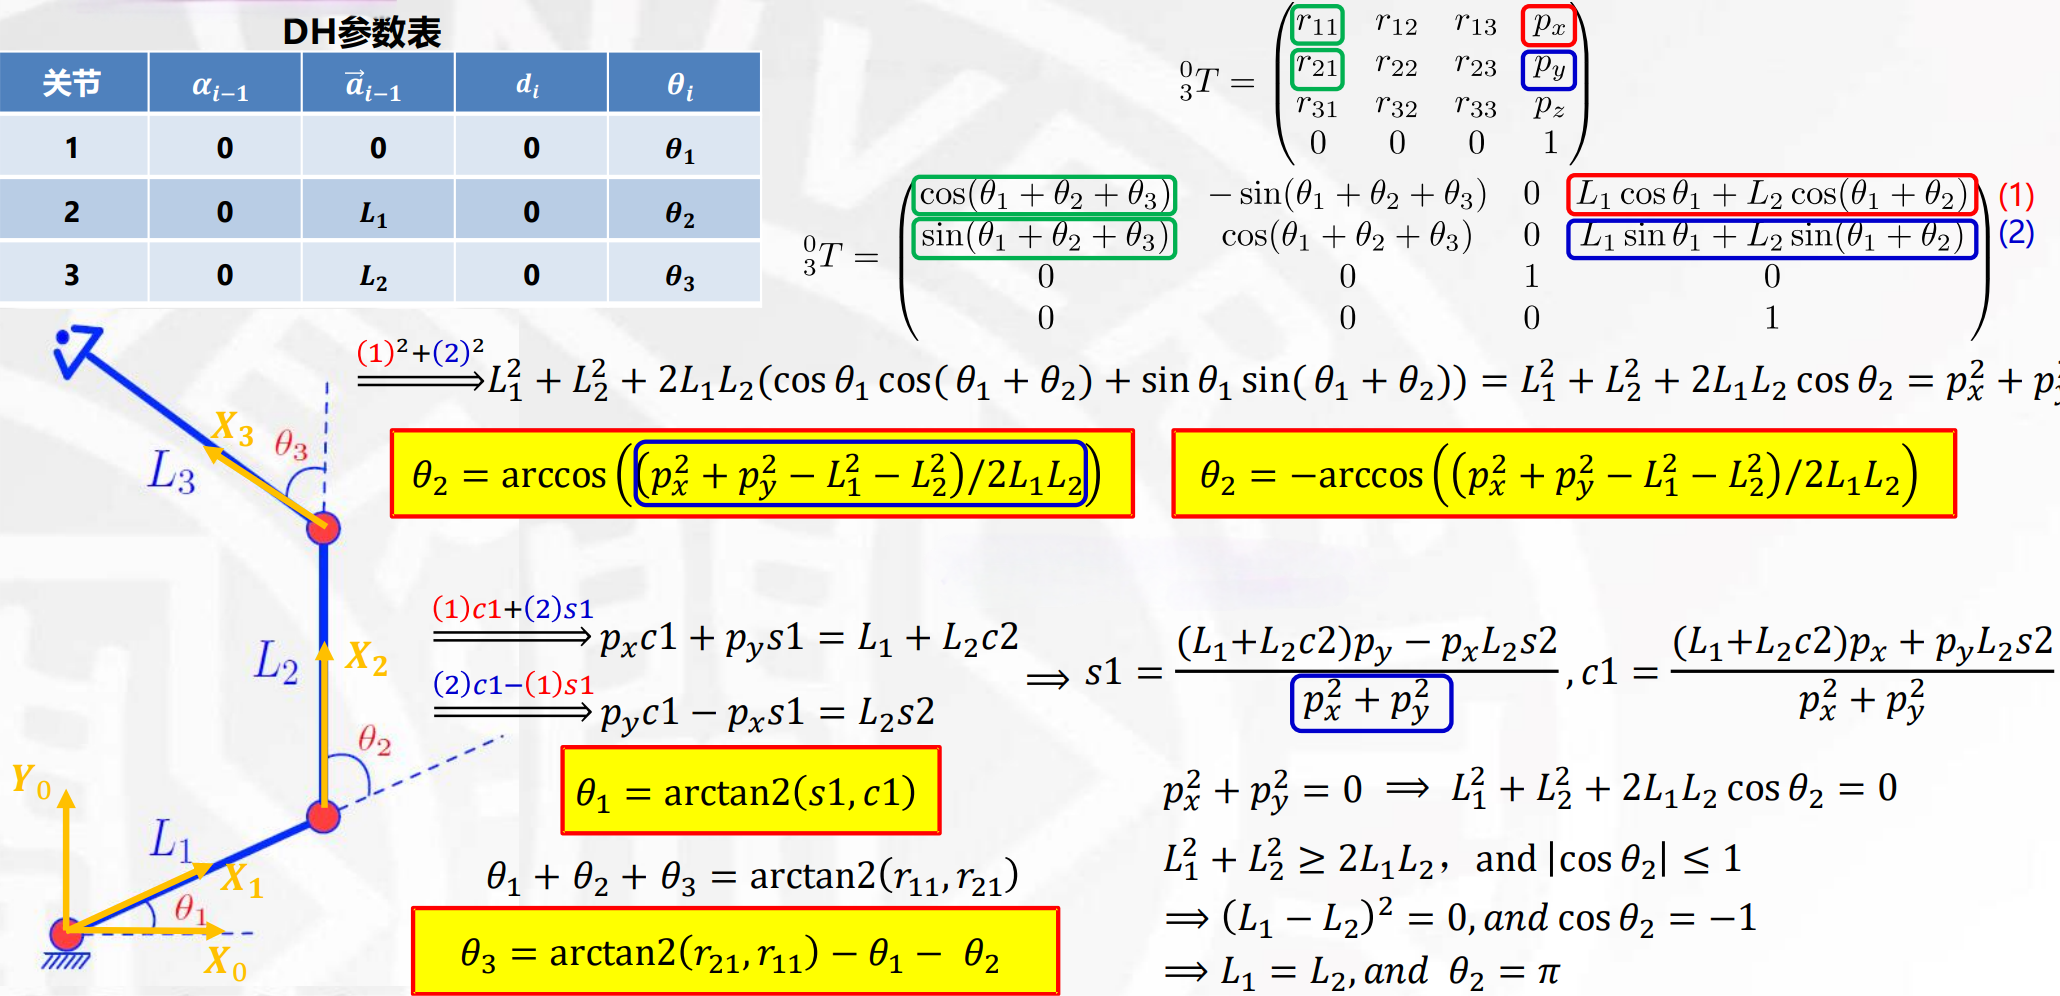
\includegraphics[width=.9\textwidth]{3.1}} \\
\subfloat[几何法]{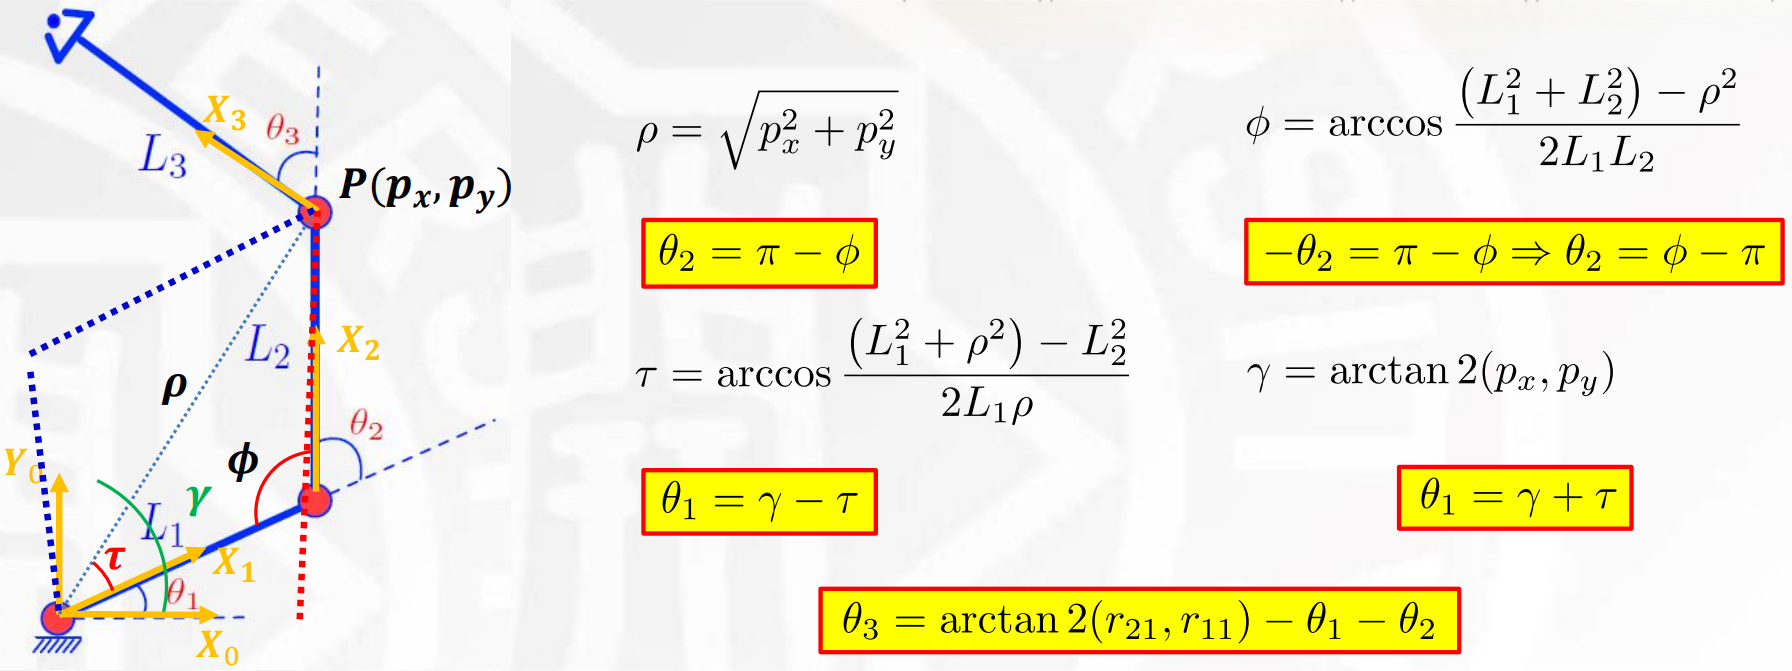
\includegraphics[width=.9\textwidth]{3.2}}
\caption[逆运动学例题1]{逆运动学例题1}
\end{figure}
%------------------------------------------------
\paragraph{例题2}\label{sec:example2.2}
{\footnotesize
接\ref{sec:example2.1},使用代数法。
}
\begin{figure}[H]
\centering 
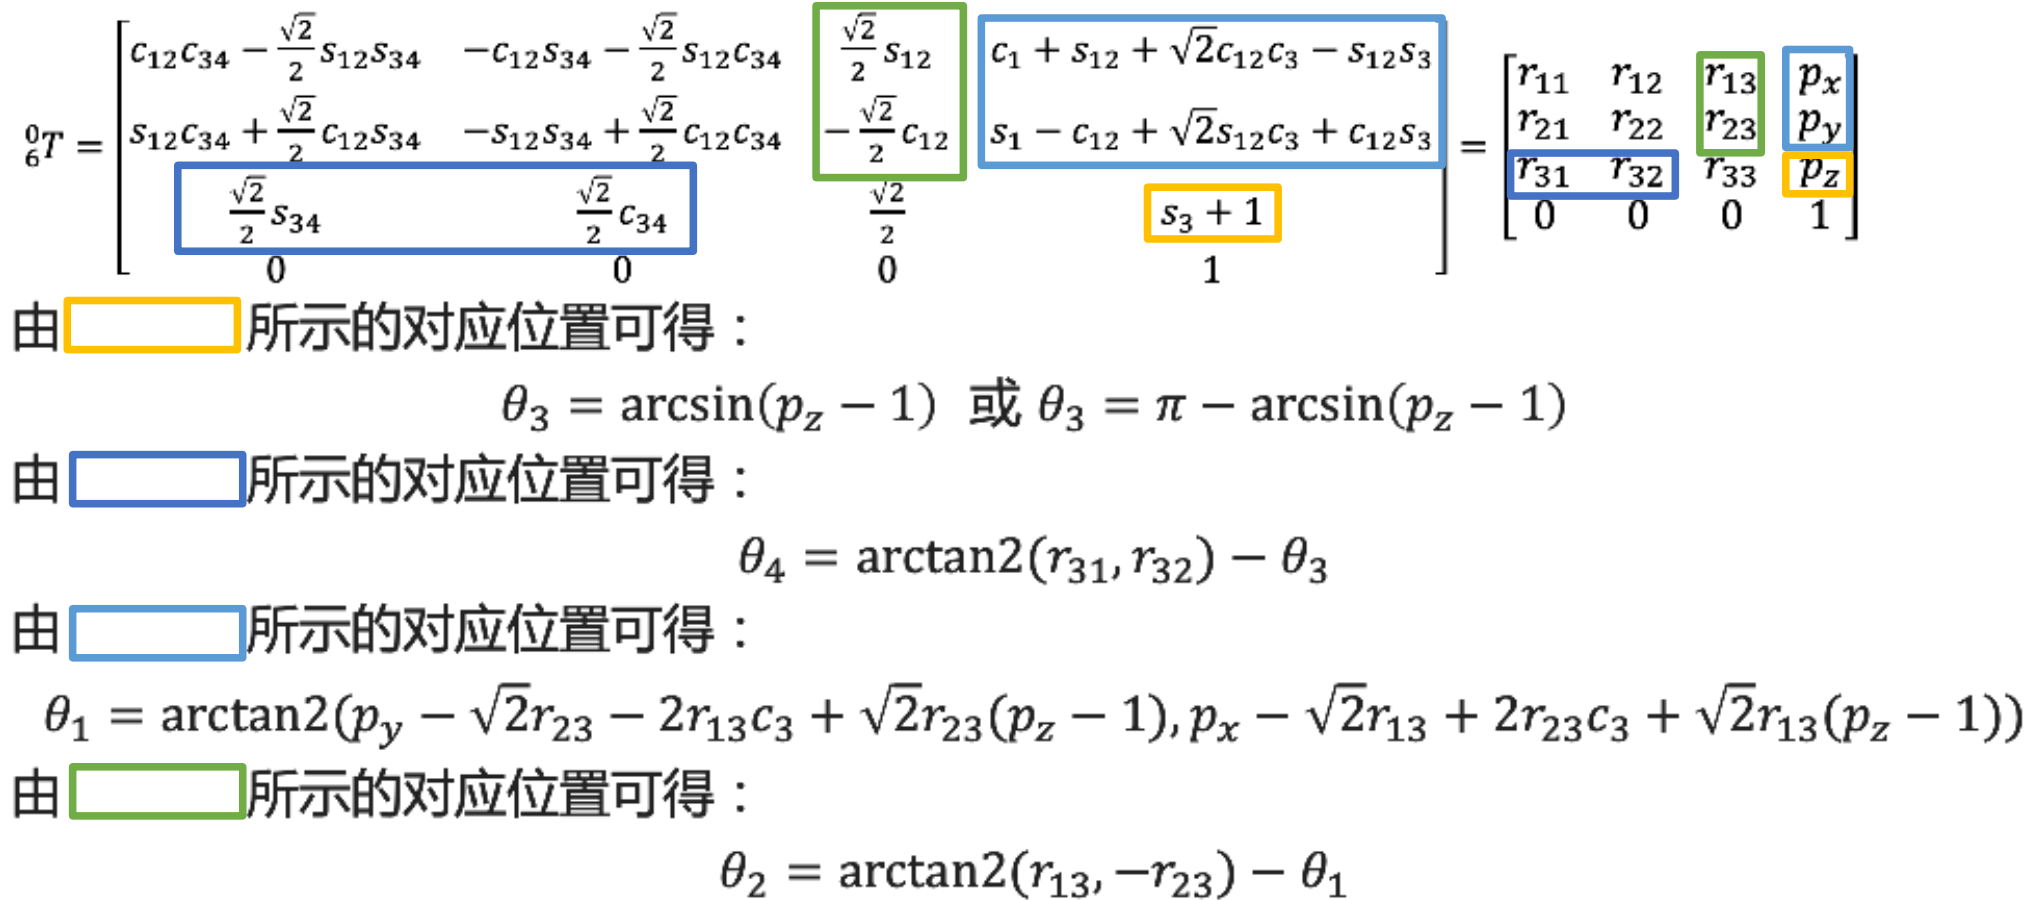
\includegraphics[width=0.8\textwidth]{2.2} 
\caption[逆运动学例题2]{逆运动学例题2}
\end{figure}
%------------------------------------------------
\subsubsection[解的讨论]{解的讨论}
\begin{itemize}
\item 存在:目标点是否超出工作空间,代数上为反三角函数定义域,几何上为三角不等式。
\item 多解:由反三角函数多解(尽量使用$ \arctan2(x, y) $保证解唯一)引起,需关注不同解对应的空间构型。
\item 奇异:自由度丢失,表现为除零。
\end{itemize} 
%------------------------------------------------
\subsection[工作空间]{工作空间}
%------------------------------------------------
\paragraph{概念}
\begin{itemize}
\item 工作空间(W):末端能到达的空间。
\item 可达空间(RW):机器人至少能以一种姿态到达的空间。
\item 灵巧空间(DW):末端能以任意姿态到达的空间。
\item $ DW \subset RW = W $。
\end{itemize} 
%------------------------------------------------
\paragraph{灵巧空间}\tip{灵巧空间}
腕部工作空间以末端执行器长为半径内外切圆。

以下以3R操作臂为例,分析不同臂长情况下的灵巧空间:
\begin{figure}[H]
\centering
\subfloat[圆环状]{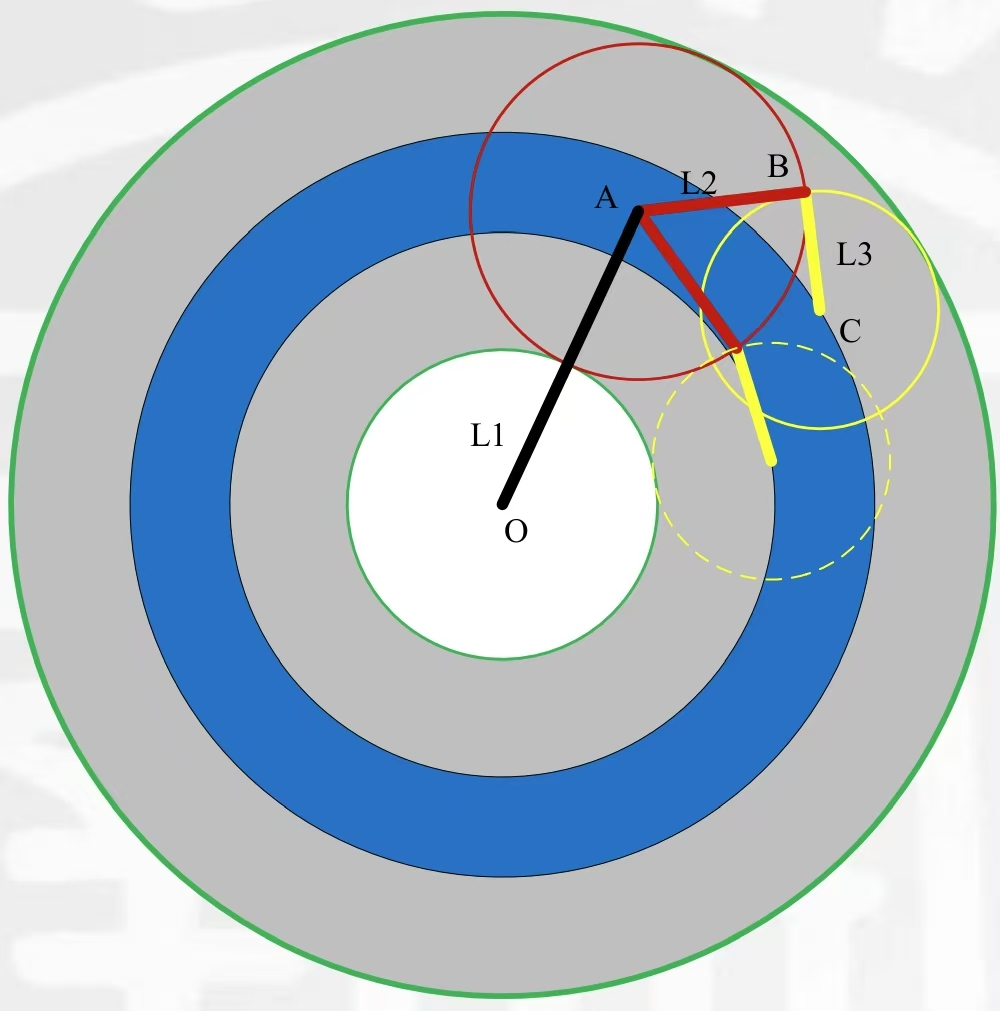
\includegraphics[width=.2\textwidth]{space1}} \quad
\subfloat[内圆外环]{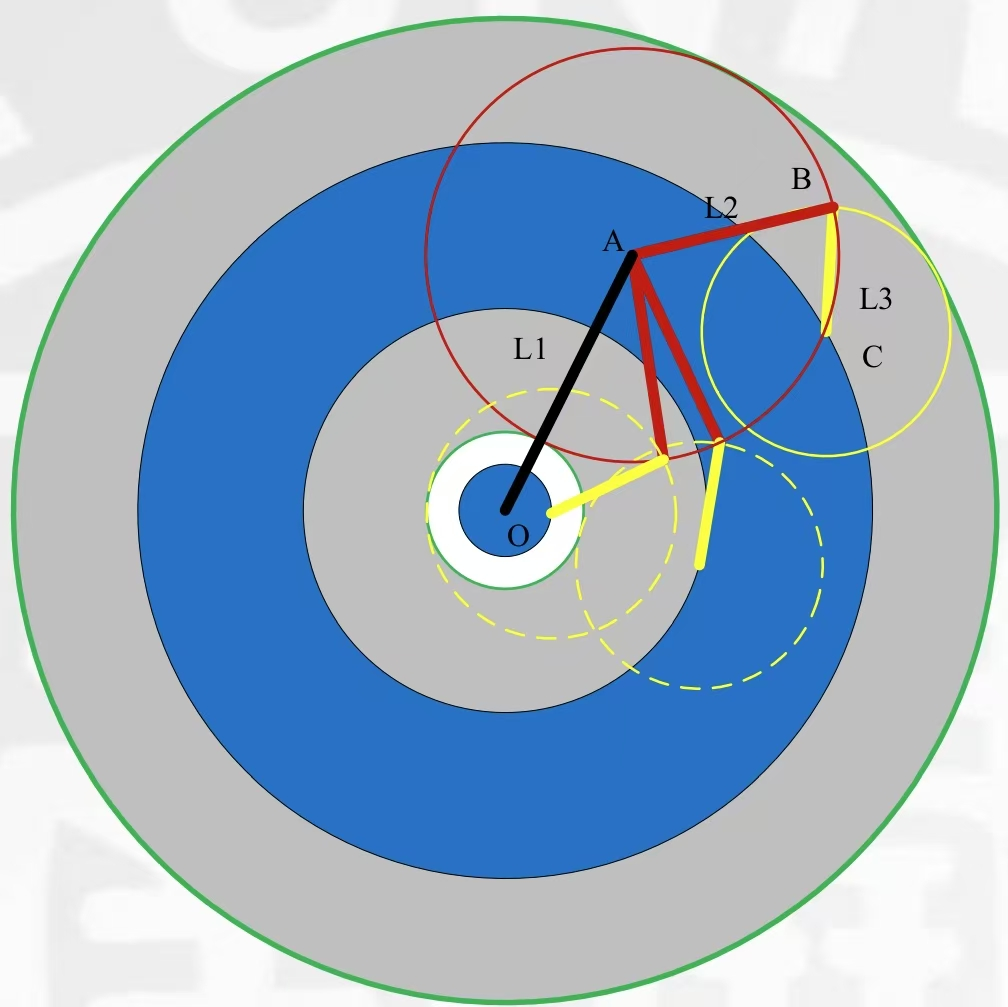
\includegraphics[width=.2\textwidth]{space2}} \quad
\subfloat[大圆]{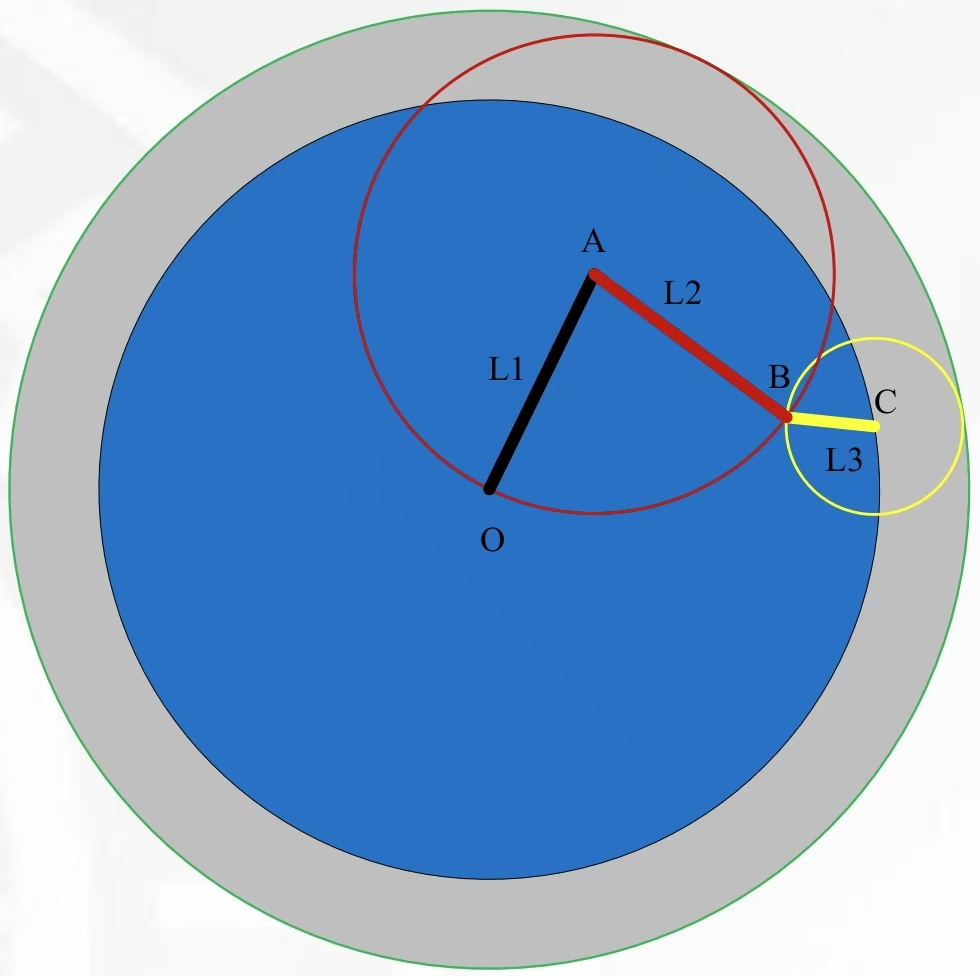
\includegraphics[width=.2\textwidth]{space5}} \\
\subfloat[内圆]{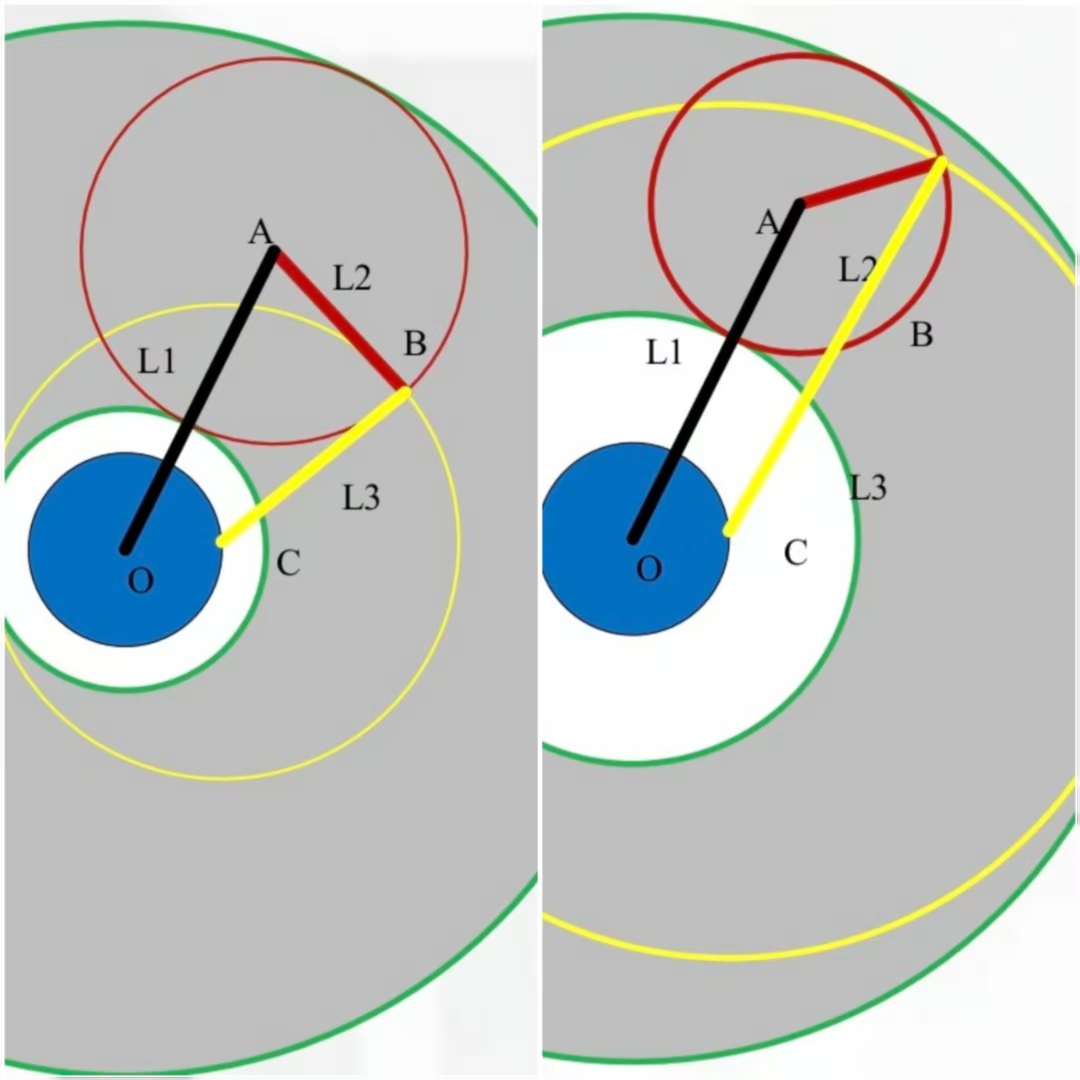
\includegraphics[width=.2\textwidth]{space3}} \quad
\subfloat[无]{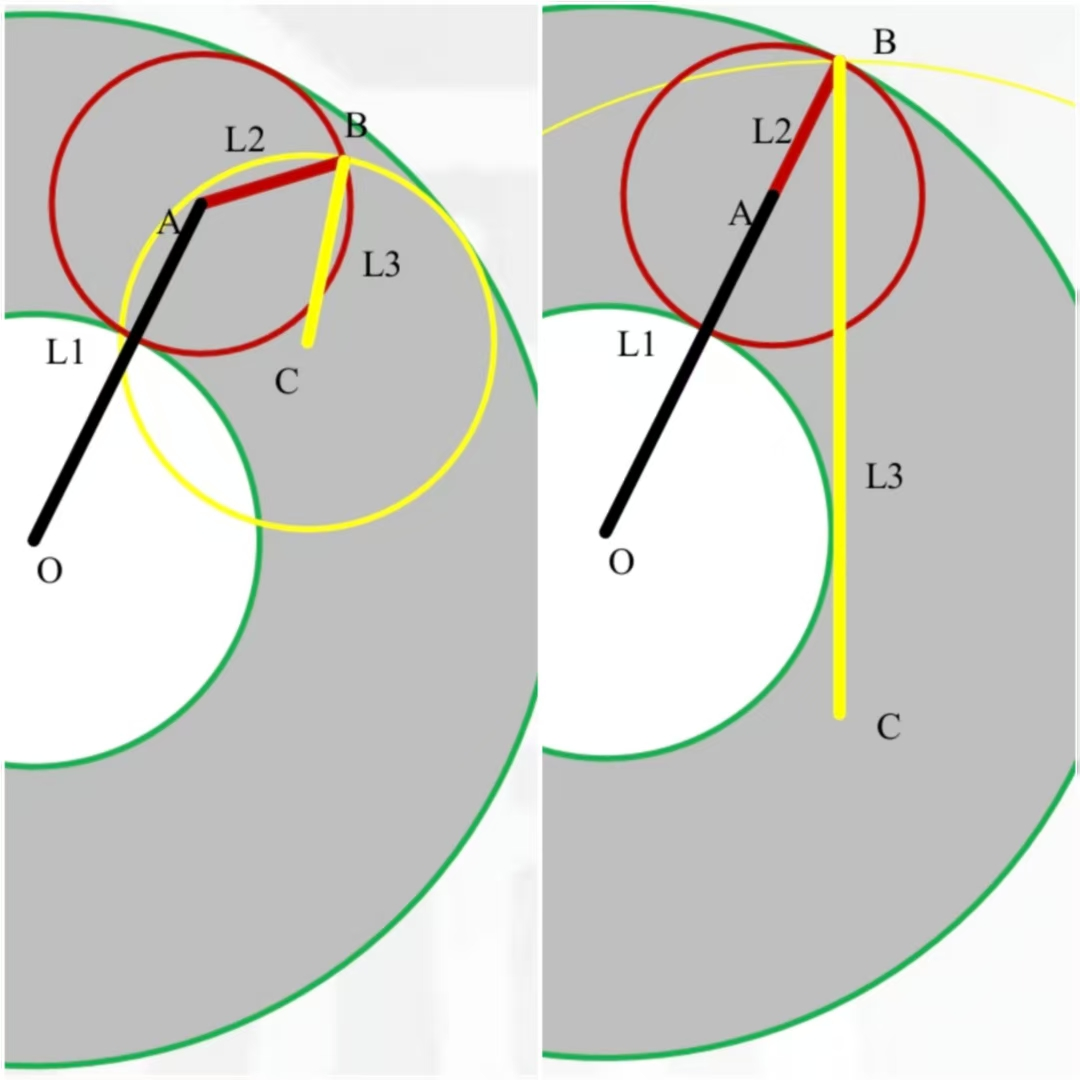
\includegraphics[width=.2\textwidth]{space4}}
\caption[3R操作臂灵巧空间]{3R操作臂灵巧空间}
\end{figure}

{\footnotesize
\begin{enumerate}
\item $ 2L_3 \leq L_1 + L_2 - |L_1 - L_2|\&L_3 \leq |L_1 - L_2| $。
\item $ 2L_3 \leq L_1 + L_2 - |L_1 - L_2|\&L_3 \geq |L_1 - L_2| $。
\item $ L_3 \leq L_1 + L_2 $。
\item $ 2L_3 \geq L_1 + L_2 - |L_1 - L_2|\&|L_1 - L_2| \leq L_3 \leq L_1 + L_2 $。
\item $ L_2 \leq L_3 \leq |L_1 - L_2|, L_3 \geq L_1 + L_2 $。
\end{enumerate}
}

为寻求较大灵巧空间,需要上下臂基本等长,且臂长不过长。
%------------------------------------------------
\paragraph{参数}
\begin{itemize}
\item $ \text{灵巧系数} = \frac{\text{可达角度所占弧长}}{\text{单位圆周长}}_{\text{(平面)}} = \frac{\text{可达角度所占表面积}}{\text{单位球表面积}}_{\text{(空间)}} $。
\item 重复精度:返回示教点精度。
\end{itemize} 
%----------------------------------------------------------------------------------------
\section{雅可比}
%------------------------------------------------
\subsection[雅可比矩阵]{雅可比矩阵}
雅可比矩阵$ J $表示关节状态(平移距离或旋转角度)$ q/\theta $变化率与末端位姿$ X $变化率关系,
$ X = f(q) $时有:
$$
\delta x_{(m \times 1)} = 
\begin{bmatrix}
\frac{\partial f_1}{\partial q_1} & \cdots & \frac{\partial f_1}{\partial q_n} \\
\vdots & \ddots & \vdots \\
\frac{\partial f_m}{\partial q_1} & \cdots & \frac{\partial f_m}{\partial q_n}
\end{bmatrix}_{(m \times n)}
\delta q_{(n \times 1)}
\Leftrightarrow 
\delta X = J(\theta)\delta \theta
$$
\begin{itemize}
\item $ J_{ij}(q) = \frac{\partial}{\partial q_j} f_i(q) $。
\item $ m $是末端位姿(输出量)描述维度,$ n $是关节变化(输入量)维度。
\end{itemize} 
%------------------------------------------------
\subsection[不同坐标描述下的雅可比矩阵转换]{不同坐标描述下的雅可比矩阵转换\tip{不同坐标描述下的雅可比矩阵转换}}
笛卡尔坐标系基础雅可比矩阵:
$$ \begin{bmatrix} v \\ \omega \end{bmatrix}_{(6 \times 1)} = J_0(q)_{(6 \times n)} \dot{q}_{(n \times 1)} $$

在不同的坐标系描述下,雅可比矩阵可以相互转化。$ X_P,X_R $定义了描述方式,$ E_P,E_R $则描述了对应的转换关系:
\begin{align*}
\dot{X}_P &= E_P \cdot v = [E_P \cdot J_v] \dot{q} = J_P \dot{q} \\
\dot{X}_R &= E_R \cdot \omega = [E_R \cdot J_\omega] \dot{q} = J_R \dot{q}
\end{align*}
$$
J = 
\begin{bmatrix} J_P \\ J_R \end{bmatrix}
=
\begin{bmatrix} E_P & 0 \\ 0 & E_R \end{bmatrix}
\begin{bmatrix} J_v \\ J_\omega \end{bmatrix}
$$
%------------------------------------------------
\paragraph{线雅可比}
\begin{itemize}
\item 柱坐标系
$
\begin{cases}
\rho = \sqrt{x^2 + y^2} \\
\theta = \arctan(y / x) \\
z = z
\end{cases}
\Rightarrow
E_P(X) =
\begin{pmatrix}
\cos\theta & \sin\theta & 0 \\
-\sin\theta / \rho & \cos\theta / \rho & 0 \\
0 & 0 & 1
\end{pmatrix}
$。
\item 球坐标系
$
\begin{cases}
\rho = \sqrt{x^2 + y^2 + z^2} \\
\theta = \arctan(\frac{y}{x}) \\
\phi = \arctan(\frac{\sqrt{x^2 + y^2}}{z})
\end{cases}
\Rightarrow
E_P(X) =
\begin{pmatrix}
\cos\theta \sin\phi & \sin\theta \sin\phi & \cos\phi \\
-\sin\theta / (\rho \sin\phi) & \cos\theta / (\rho \sin\phi) & 0 \\
\cos\theta \cos\phi / \rho & \sin\theta \cos\phi / \rho & -\sin\phi / \rho
\end{pmatrix}
$。
\end{itemize} 
%------------------------------------------------
\paragraph{角雅可比}
\begin{itemize}
\item 旋转阵推基础\label{sec:Rotation_matrix}

旋转阵导数为
$ \dot{R} = \lim_{\Delta t \to 0} (\frac{R_K(\Delta\theta) - I_3}{\Delta t} R(t)) $,

其与逆(转置)的积为反对称阵
$ \dot{R} R^{-1} = \dot{R} R^T = \hat{\Omega} = \begin{bmatrix} 0 & -\Omega_z & \Omega_y \\ \Omega_z & 0 & -\Omega_x \\ -\Omega_y & \Omega_x & 0 \end{bmatrix} $

得到
$
\begin{cases}
\Omega_x = \dot{r}_{31} r_{21} + \dot{r}_{32} r_{22} + \dot{r}_{33} r_{23} \\
\Omega_y = \dot{r}_{11} r_{31} + \dot{r}_{12} r_{32} + \dot{r}_{13} r_{33} \\
\Omega_z = \dot{r}_{21} r_{11} + \dot{r}_{22} r_{12} + \dot{r}_{23} r_{13}
\end{cases}
$,

$ \Omega = \begin{bmatrix} \Omega_x & \Omega_y & \Omega_z \end{bmatrix}^T = \begin{bmatrix} k_x & k_y & k_z \end{bmatrix}^T $为瞬时旋转轴。

例题\ref{sec:example4.2}。
\item 基础推旋转角

对于Z-Y-Z欧拉角(X-Y-Z固定角)$ X_R = \begin{bmatrix} \alpha & \beta & \gamma \end{bmatrix}^T $,有旋转阵:
$$
^A_B R(\alpha, \beta, \gamma) =
\begin{bmatrix}
c\alpha c\beta c\gamma - s\alpha s\gamma & -c\alpha c\beta s\gamma - s\alpha c\gamma & c\alpha s\beta \\
s\alpha c\beta c\gamma + c\alpha s\gamma & -s\alpha c\beta s\gamma + c\alpha c\gamma & s\alpha s\beta \\
-s\beta c\gamma & s\beta s\gamma & c\beta
\end{bmatrix}
$$

变换为:
$$
\begin{bmatrix} \Omega_x \\ \Omega_y \\ \Omega_z \end{bmatrix}
=
\begin{bmatrix} 0 & -s\alpha & c\alpha s\beta \\ 0 & c\alpha & s\alpha s\beta \\ 1 & 0 & c\beta \end{bmatrix}
\begin{bmatrix} \dot{\alpha} \\ \dot{\beta} \\ \dot{\gamma} \end{bmatrix}
\Rightarrow 
\begin{bmatrix} \dot{\alpha} \\ \dot{\beta} \\ \dot{\gamma} \end{bmatrix}
=
\underbrace{\begin{bmatrix}
\frac{c\alpha c\beta}{s\beta} & -\frac{s\alpha c\beta}{s\beta} & 1 \\
-\frac{s\alpha}{s\beta} & \frac{c\alpha}{s\beta} & 0 \\
c\alpha & s\alpha & 0
\end{bmatrix}}_{E_R}
\begin{bmatrix} \Omega_x \\ \Omega_y \\ \Omega_z \end{bmatrix}
$$
\end{itemize} 
%------------------------------------------------
\subsection[求导法]{求导法\tip{求导求雅可比}}
\begin{itemize}
\item 直接法:对正运动学方程直接求导。
$$ J = \begin{bmatrix} \frac{\partial X_P}{\partial q_1} & \frac{\partial X_P}{\partial q_2} & \cdots & \frac{\partial X_P}{\partial q_N} \\ \frac{\partial x_R}{\partial q_1} & \frac{\partial x_R}{\partial q_2} & \cdots & \frac{\partial x_R}{\partial q_N} \end{bmatrix} $$
\item 旋转阵法:线雅可比直接求导,角雅可比提取各旋转阵$ Z $列(原理见\ref{sec:Terminal_function})。\label{sec:Terminal_function_back}
\end{itemize} 
$$ J = \begin{bmatrix} \frac{\partial X_P}{\partial q_1} & \frac{\partial X_P}{\partial q_2} & \cdots & \frac{\partial X_P}{\partial q_N} \\ \overline{\epsilon}_1 Z_1 & \overline{\epsilon}_2 Z_2 & \cdots & \overline{\epsilon}_n Z_n \end{bmatrix} $$
%------------------------------------------------
\paragraph{例题1}
{\footnotesize
以下以斯坦福臂(2RP3R)为例:

\begin{figure}[H]
\centering
\subfloat[斯坦福臂结构图]{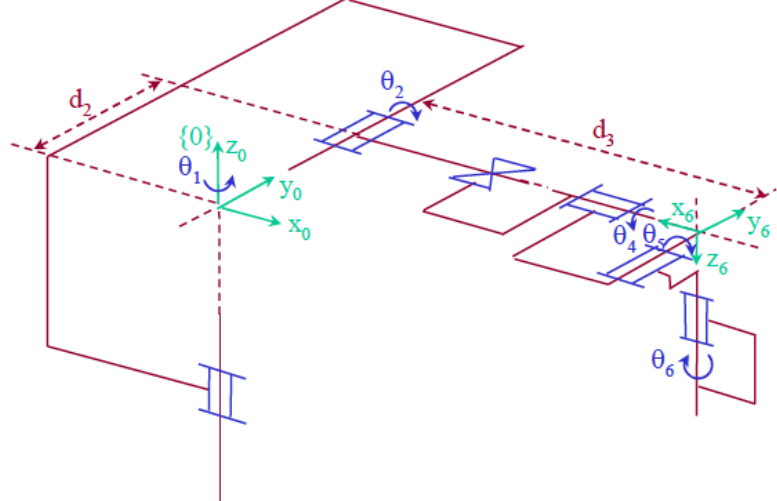
\includegraphics[width=.45\textwidth]{4.1}} \quad
\subfloat[参数表]{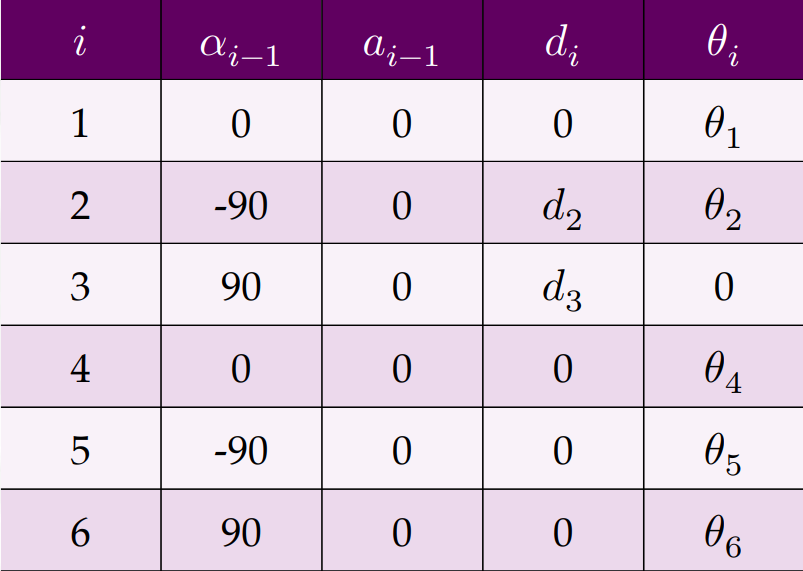
\includegraphics[width=.45\textwidth]{4.2}}
\caption[旋转阵法求雅可比例题]{旋转阵法求雅可比例题}
\end{figure}

$ _6^0T = {_1^0T}{_2^1T}{_3^2T}{_4^3T}{_5^4T}{_6^5T} $得到正运动学方程,将其提取为列向量:
$$
X = \begin{bmatrix} X_P \\ r_1 \\ r_2 \\ \textcolor{red}{r_3} \end{bmatrix}
=
\begin{bmatrix}
d_3 c_1 s_2 - d_2 s_1 \\
d_3 s_1 s_2 + d_2 c_1 \\
d_3 c_2 \\
{r_1}_{(3 \times 1)} \\
{r_2}_{(3 \times 1)} \\
\textcolor{red}{c_1(c_2 c_4 s_5 + s_2 c_5) - s_1 s_4 s_5} \\
\textcolor{red}{s_1(c_2 c_4 s_5 + s_2 c_5) + c_1 s_4 s_5} \\
\textcolor{red}{-s_2 c_4 s_5 + c_2 c_5}
\end{bmatrix}
$$

雅可比矩阵为:
\begin{align*}
J &= \begin{bmatrix} Z_1 \times P_{13} & Z_2 \times P_{23} & Z_3 & Z_4 \times 0 & Z_5 \times 0 & Z_6 \times 0 \\ Z_1 & Z_2 & 0 & Z_4 & Z_5 & Z_6 \end{bmatrix}
= \begin{bmatrix} \frac{\partial X_P}{\partial q_1} & \frac{\partial X_P}{\partial q_2} & \frac{\partial X_P}{\partial q_3} & 0 & 0 & 0 \\ Z_1 & Z_2 & 0 & Z_4 & Z_5 & \textcolor{red}{Z_6} \end{bmatrix} \\
&=
\begin{bmatrix}
-(d_3 s_1 s_2 + d_2 c_1) & c_1 c_2 d_3 & c_1 s_2 & 0 & 0 & 0 \\
d_3 c_1 s_2 - d_2 s_1 & s_1 c_2 d_3 & s_1 s_2 & 0 & 0 & 0 \\
0 & -s_2 d_3 & c_2 & 0 & 0 & 0 \\
0 & -s_1 & 0 & c_1 s_2 & -c_1 c_2 s_4 - s_1 c_4 & \textcolor{red}{c_1 c_2 c_4 s_5 - s_1 s_4 s_5 + c_1 s_2 c_5} \\
0 & c_1 & 0 & s_1 s_2 & -s_1 c_2 s_4 + c_1 c_4 & \textcolor{red}{s_1 c_2 c_4 s_5 + c_1 s_4 s_5 + s_1 s_2 c_5} \\
1 & 0 & 0 & c_2 & s_2 s_4 & \textcolor{red}{-s_2 c_4 s_5 + c_2 c_5}
\end{bmatrix}
\end{align*}

以上省略了中间的齐次变换阵,它们旋转阵$ Z $列对应各$ Z_i $。

在$ \theta_5 = k\pi $时,奇异,简化为(第4列和第6列相同):
$$
\begin{bmatrix}
x & x & x& 0 & 0 & 0 \\
x & x & x & 0 & 0 & 0 \\
x & x & x& 0 & 0 & 0 \\
0 & x & 0 & c_1 s_2 & x & c_1 s_2 \\
0 & x & 0 & s_1 s_2 & x & s_1 s_2 \\
x & 0 & 0 & c_2 & x& c_2
\end{bmatrix}
$$
}
%------------------------------------------------
\paragraph{例题2}\label{sec:example4.2}
{\footnotesize
3R机器人正运动学齐次变换阵为:
$$ \begin{bmatrix} c_1c_{23} & -c_1s_{23} & s_1 & l_1c_1 + l_2c_1c_2 \\ s_1c_{23} & -s_1s_{23} & -c_1 & l_1s_1 + l_2s_1c_2 \\ s_{23} & c_{23} & 0 & l_2s_2 \\ 0 & 0 & 0 & 1 \end{bmatrix} $$

对平移向量和旋转阵分别求偏导,得到:
\begin{align*}
^0J_v(\theta) &= \begin{bmatrix} -l_1s_1 - l_2s_1c_2 & -l_2c_1s_2 & 0 \\ l_1c_1 + l_2c_1c_2 & -l_2s_1s_2 & 0 \\ 0 & l_2c_2 & 0 \end{bmatrix} \\
^0J_R(\theta) &= \begin{bmatrix}
-s_1c_{23} & -c_1s_{23} & -c_1s_{23} \\ s_1s_{23} & -c_1c_{23} & -c_1c_{23} \\ c_1 & 0 & 0 \\
c_1c_{23} & -s_1s_{23} & -s_1s_{23} \\ -c_1s_{23} & -s_1c_{23} & -s_1c_{23} \\ s_1 & 0 & 0 \\
0 & c_{23} & c_{23} \\ 0 & -s_{23} & -s_{23} \\ 0 & 0 & 0
\end{bmatrix}
\end{align*}

可转化$ ^0J_R(\theta) $为基础角雅可比(见\ref{sec:Rotation_matrix}),结果略。
}
%------------------------------------------------
\subsection[速度传播法]{速度传播法}
%------------------------------------------------
\subsubsection[串行逐连杆求解]{串行逐连杆求解\tip{串行速度传播求雅可比}}
由连杆$ k $起始端速度,求其末端速度,进而获得连杆$ k + 1 $起始端速度。
\begin{figure}[H]
\centering 
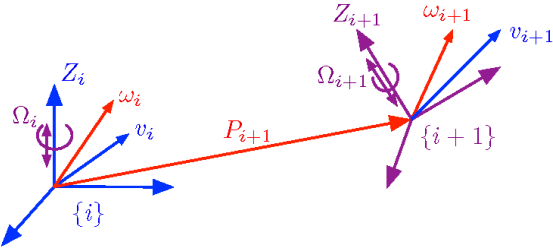
\includegraphics[width=0.5\textwidth]{Velocity propagation} 
\caption[串行速度传播]{串行速度传播}
\end{figure}

\begin{itemize}
\item 平移关节:线速度传导+角速度转换线速度+平移变化。
$$
v_{i + 1} = v_i + \omega_i \times P_{i + 1} + \dot{d}_{i + 1} \cdot Z_{i + 1}
\overset{\text{换系}}{\Longrightarrow}
{}^{i + 1}v_{i + 1} = ^{i + 1}_i R \cdot (^i v_i + ^i\omega_i \times ^i P_{i + 1}) + \dot{d}_{i + 1} \cdot ^{i + 1}Z_{i + 1}
$$
\item 旋转关节:角速度传导+旋转变化。
$$
\Omega_{i + 1} = \dot{\theta}_{i + 1} \cdot Z_{i + 1}, \omega_{i + 1} = \omega_i + \Omega_{i + 1}
\overset{\text{换系}}{\Longrightarrow}
{}^{i + 1}\omega_{i + 1} = ^{i + 1}_i R \cdot ^i\omega_i + \dot{\theta}_{i + 1} \cdot ^{i + 1}Z_{i + 1}
$$
\end{itemize} 
%------------------------------------------------
\subsubsection[并行末端作用求解]{并行末端作用求解\tip{并行速度传播求雅可比}}
%------------------------------------------------
\paragraph{单关节作用}\label{sec:bingxing}
求一关节运动对末端运动影响时,将其他连杆固定,视为刚体。
\begin{figure}[H]
\centering 
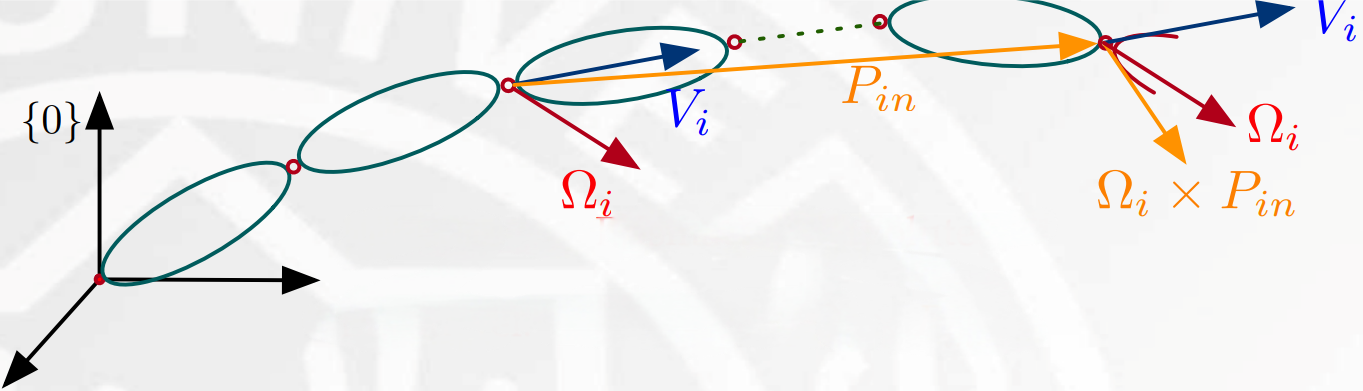
\includegraphics[width=0.6\textwidth]{Terminal function} 
\caption[并行速度传播]{并行速度传播}
\end{figure}

\begin{table}[H]
\centering
\begin{tabular}{c|cc}
\hline
& 平移关节 & 旋转关节 \\
\hline
线速度 & $ V_i $ & $ \Omega_i \times P_{in} $ \\
角速度 & $ 0 $ & $ \Omega_i $ \\
\hline
\end{tabular}
\caption{并行速度传播}
\end{table}

\begin{itemize}
\item 线速度由线速度传导和角速度转换线速度组成。
\item 角速度只有角速度传导。
\end{itemize} 

回到雅可比转换\ref{sec:bingxing_back1},回到惯性阵$ M(q) $求取\ref{sec:bingxing_back2}。
%------------------------------------------------
\paragraph{综合作用}\label{sec:Terminal_function}
基于基坐标系,由$ V_i = Z_i \dot{q}_i, \Omega_i = Z_i \dot{q}_i $,综合各关节运动,得到:
\begin{align*}
v &= \sum_{i = 1}^n [\epsilon_i V_i + \overline{\epsilon}_i (\Omega_i \times P_{in})] = \sum_{i = 1}^n [\epsilon_i Z_i + \overline{\epsilon}_i (Z_i \times P_{in})] \dot{q}_i \\
\omega &= \sum_{i = 1}^n \overline{\epsilon}_i \Omega_i = \sum_{i = 1}^n (\overline{\epsilon}_i Z_i) \dot{q}_i
\end{align*}

回到旋转阵法\ref{sec:Terminal_function_back}。
%------------------------------------------------
\subsection[静态力传播法]{静态力传播法\tip{静态力传播求雅可比}}
%------------------------------------------------
\subsubsection[静态力与力矩]{静态力与力矩}\label{sec:fn1}
由末端往回推,根据各连杆力与力矩平衡进行求解。

对于连杆$ i $,$ f_i, n_i $表示自身受力(矩),$ -f_{i + 1}, -n_{i + 1} $表示下一连杆的反作用力(矩),$ P $表示其长度,有:
$$
\begin{cases}
f_i = f_{i + 1} \\
n_i = n_{i + 1} + P_{i + 1} \times f_{i + 1}
\end{cases}
\overset{\text{换系}}{\Longrightarrow}
\begin{cases}
^i f_i = ^i_{i + 1}R \cdot ^{i + 1} f_{i + 1} \\
^i n_i = ^i_{i + 1}R \cdot ^{i + 1} n_{i + 1} + ^i P_{i + 1} \times ^i f_i
\end{cases}
$$

与动力学受力分析对比\ref{sec:fn2}

\begin{figure}[H]
\centering
\subfloat[静力学受力分析]{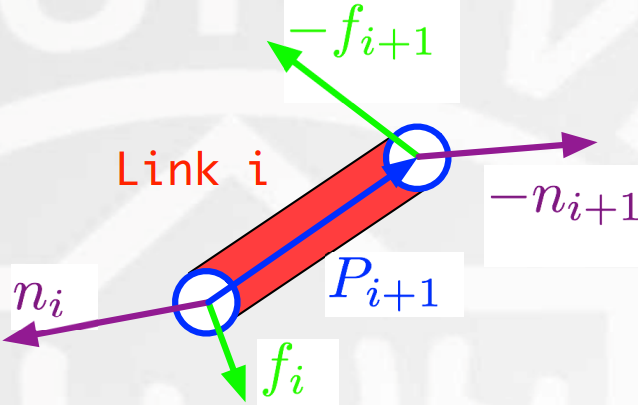
\includegraphics[width=.25\textwidth]{force}} \quad
\subfloat[平移关节]{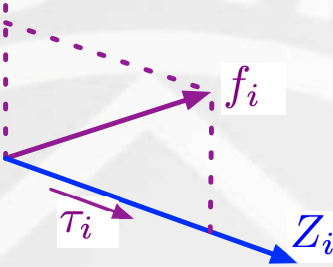
\includegraphics[width=.2\textwidth]{Prismatic Joint}} \quad
\subfloat[旋转关节]{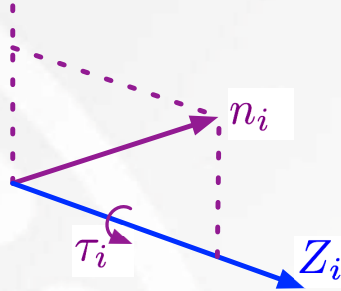
\includegraphics[width=.2\textwidth]{Revolute Joint}}
\caption[静态力与力矩]{静态力与力矩}
\end{figure}

\begin{table}[H]
\centering
\begin{tabular}{c|cc}
\hline
& 平移关节 & 旋转关节 \\
\hline
计算量 & 力 & 力矩 \\
计算 & $ \tau_i = f_i^T Z_i $ & $ \tau_i = n_i^T Z_i $ \\
内部平衡量 & 力矩 & 力 \\
\hline
\end{tabular}
\caption{力与力矩(动静一致)}
\end{table}
%------------------------------------------------
\subsubsection[速度与扭矩]{速度与扭矩}
\begin{figure}[H]
\centering
\subfloat[角速度与线速度]{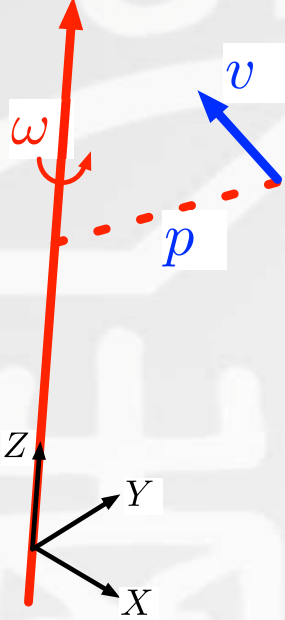
\includegraphics[width=.125\textwidth]{wv}} \quad
\subfloat[力与扭矩]{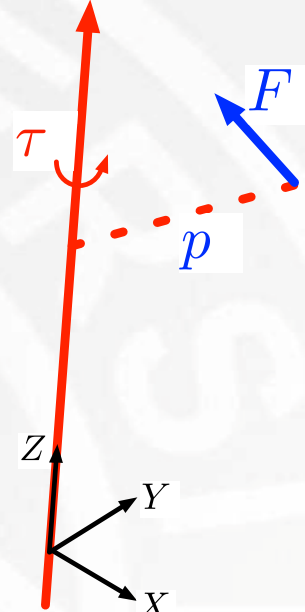
\includegraphics[width=.125\textwidth]{ft}}
\caption[速度与扭矩]{速度与扭矩}
\end{figure}

\begin{align*}
v &= \omega \times p = -\hat{p} \omega = J \dot{\theta} \\
\tau &= p \times F = -\hat{p}^T F = J^T F
\end{align*}
%------------------------------------------------
\subsubsection[虚功原理]{虚功(Virtual Work)原理\tip{虚功原理}}
已知各连杆力(矩),微小移动$ \delta x $下,各力(矩)作功之和为$ \delta W = \sum_i f_i \delta x_i $,在其等于$ 0 $时,各力(矩)所作功抵消,即:
$$ \tau^T \delta q + (-F)^T \delta x = 0 $$

因为$ \delta x = J \delta q $,所以$ \tau = J^T F $。

这里$ J $是末端雅可比,而非腕部雅可比。
%------------------------------------------------
\paragraph{例题}
\begin{figure}[H]
\centering 
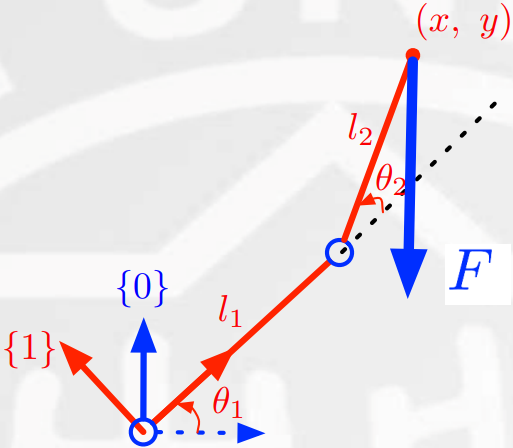
\includegraphics[width=0.25\textwidth]{5} 
\caption[虚功原理例题]{虚功原理例题}
\end{figure}
{\footnotesize
条件: $ l_1 = l_2 = 1, \theta_1 = 0, \theta_2 = 60^\circ, F = \begin{bmatrix} 0 & -1 & 0 \end{bmatrix}^T N $。
\begin{enumerate}
\item 对于连杆2:$ f_2 = F, n_2 = \vec{l}_2 \times F = \begin{bmatrix} 0 & 0 & -l_2 \cos(\theta_1 + \theta_2) \end{bmatrix}^T N $。
\item 对于连杆1:$ f_1 = f_2 = F, n_1 = n_2 + \vec{l}_1 \times f_2 = \begin{bmatrix} 0 & 0 & -l_1 \cos\theta_1 - l_2 \cos(\theta_1 + \theta_2) \end{bmatrix}^T N $。
\item 根据$ \dot{x} = J \dot{\theta} $,由几何关系得$ J = \begin{bmatrix} -(l_1 s_1 + l_2 s_{12}) & -l_2 s_{12} \\ l_1 c_1 + l_2 c_{12} & l_2 c_{12} \end{bmatrix} $。
\item 因此$ \tau = J^T F = \begin{bmatrix} -(l_1 s_1 + l_2 s_{12}) & l_1 c_1 + l_2 c_{12} \\ - l_2 s_{12} & l_2 c_{12} \end{bmatrix} \begin{bmatrix} 0 \\ -1 \end{bmatrix} $。
\end{enumerate}
}
%------------------------------------------------
\subsection[雅可比转换]{雅可比转换\tip{雅可比转换}}\label{sec:Jacobian transform}\label{sec:bingxing_back1}
一般求解基坐标系下的腕部雅可比$ ^0 J_j $。
%------------------------------------------------
\paragraph{位置转换}
根据并行求解结论(见\ref{sec:bingxing}),换序+反对称:
$$ 
\begin{bmatrix} v_j \\ \omega_j \end{bmatrix} 
=
\begin{bmatrix} E & -\hat{P}_{ij} \\ 0 & E \end{bmatrix}
\begin{bmatrix} v_i \\ \omega_i \end{bmatrix} 
\Rightarrow 
J_j = \begin{bmatrix} E & -\hat{P}_{ij} \\ 0 & E \end{bmatrix} J_i
$$ 
%------------------------------------------------
\paragraph{坐标系转换}
$ ^0\hat{P}_{ij} = ^0_n R \cdot ^n\hat{P}_{ij} \cdot ^0_n R^T $:
$$ ^0 J_j = \begin{bmatrix} ^0_n R & -^0_n R \cdot ^n\hat{P}_{ij} \cdot ^0_n R^T \\ 0 & ^0_n R \end{bmatrix} {}^n J_i $$
%------------------------------------------------
\subsection[其他]{其他}
%------------------------------------------------
\subsubsection[雅可比奇异]{雅可比奇异\tip{雅可比奇异}}
\begin{itemize}
\item 不同坐标系下雅可比矩阵不同,但是行列式相同,$ ^i J \neq ^j J, |^i J| = |^j J| $。
\item $ |J(q)| = 0 $时,奇异,存在方向无法运动或旋转,控制失效。
\end{itemize} 
%------------------------------------------------
\subsubsection[雅可比速率控制]{雅可比速率控制}
\begin{figure}[H]
\centering 
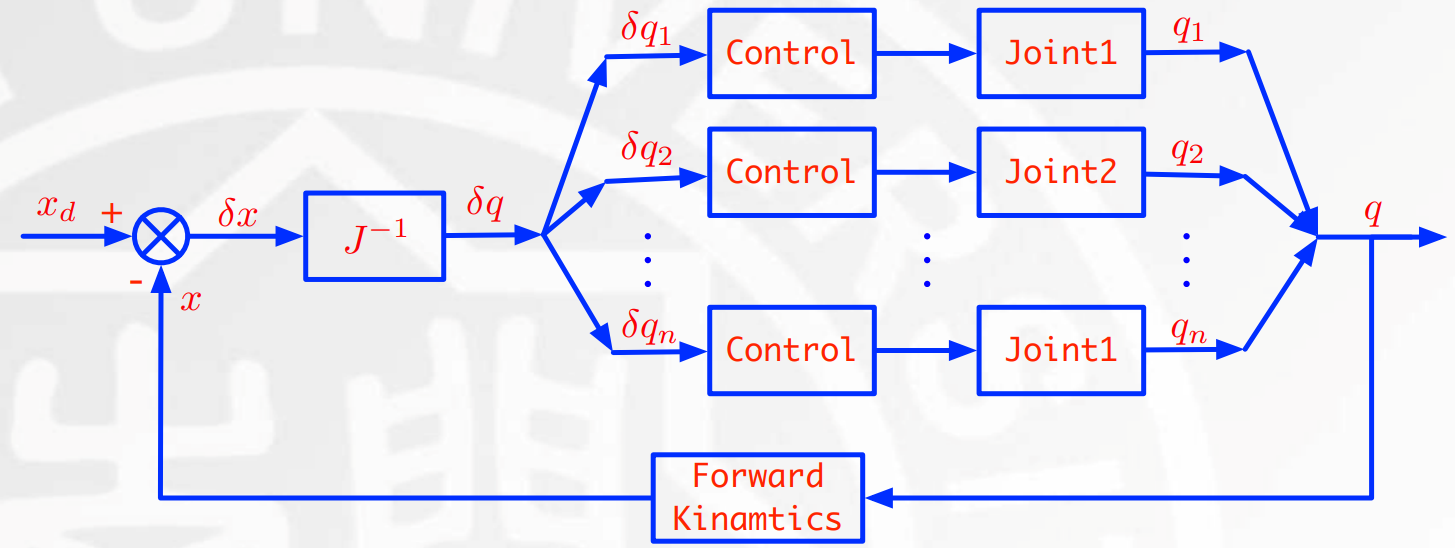
\includegraphics[width=0.6\textwidth]{J_control} 
\caption[雅可比速率控制]{雅可比速率控制}
\end{figure}

$ \delta q = J(q)^{-1} \delta x $,为保证可逆,可采用伪逆$ J(q)^+ $。
%------------------------------------------------
\section{动力学}
%------------------------------------------------
\subsection[刚体动力学]{刚体动力学}
%------------------------------------------------
\subsubsection[受力种类分析]{受力种类分析}
\begin{itemize}
\item 惯性参考系
\begin{itemize}
\item 重力$ G $。
\item 惯性力$ F_1 = ma $。
\end{itemize} 
\item 旋转参考系(非惯性参考系):假想力。
\begin{itemize}
\item 离心力$ F_2 = m\omega^2r $:沿半径背离圆心。
\item 科里奥利力$ F_3 = 2mv' \times \omega $:相对于参考系运动的惯性力(在惯性参考系下表现为物体保持直线运动)。
\end{itemize} 
\item 合力:$ \Gamma = ma + m\omega^2r + 2mv' \times \omega + G = M(q)\ddot{q} + V(q, \dot{q}) + G(q) $。 \\
其中,$ \Gamma $为广义关节力,$ q,\dot{q},\ddot{q} $为关节空间坐标、速度、加速度,$ M(q) $为惯性阵。
\end{itemize} 
%------------------------------------------------
\subsubsection[运动分析]{运动分析\tip{运动分析}}
\begin{figure}[H]
\centering
\subfloat[质点直线运动]{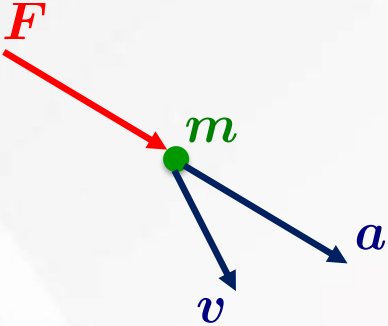
\includegraphics[width=.15\textwidth]{point_p}} \quad
\subfloat[刚体直线运动]{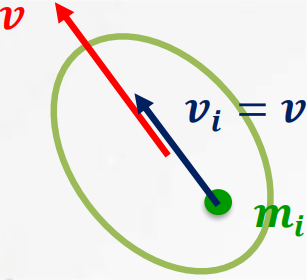
\includegraphics[width=.15\textwidth]{rigid_p}} \quad
\subfloat[质点旋转运动]{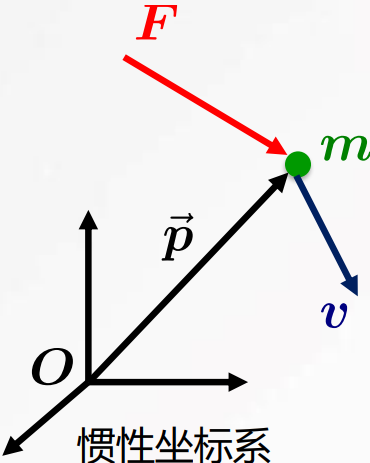
\includegraphics[width=.15\textwidth]{point_r}} \quad
\subfloat[刚体旋转运动]{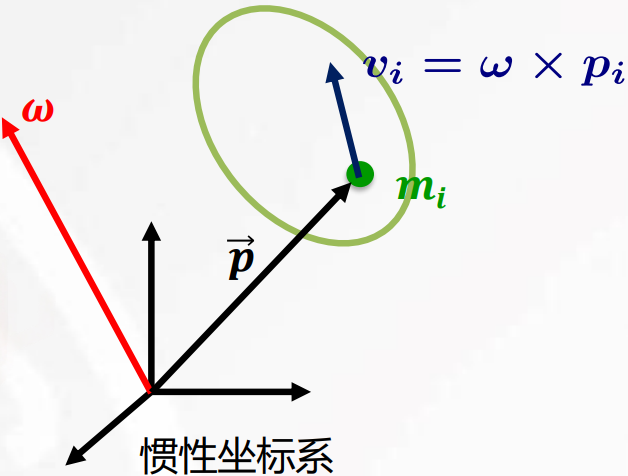
\includegraphics[width=.2\textwidth]{rigid_r}}
\caption[运动分析]{运动分析}
\end{figure}
%------------------------------------------------
\paragraph{直线运动}
\begin{itemize}
\item 动量守恒(合外力为零,系统总动量不变):$ F = ma = m\dot{v} = \dot{Q} $。
\item 动量变化率等于所受外力:
$$ 
Q = mv
\overset{\text{质点到刚体}}{\Longrightarrow}
Q = \int_V v_i \rho dV = (\int_V \rho dV) v = mv
$$
质量$ m = diag(m,m,m) $表明刚体空间运动的各向同性。
\end{itemize} 
%------------------------------------------------
\paragraph{旋转运动}
\begin{itemize}
\item 角动量守恒(合外力为零/指向原点,系统总角动量不变):$ \tau = \vec{p} \times m\dot{v} = \dot{L} $。
\item 角动量变化量等于所受外力矩:
$$ 
L = \vec{p} \times mv = mp \times (\omega \times p)
\overset{\text{质点到刚体}}{\Longrightarrow}
L = \int_V p \times (\omega \times p) \rho dV = (\int_V -\hat{p}\hat{p}\rho dV) \omega = I\omega 
$$
\end{itemize} 
%------------------------------------------------
\subsubsection[惯性张量]{惯性张量$ I $\tip{惯性张量}}
%------------------------------------------------
\paragraph{计算}
$$
-\hat{p}\hat{p} = (p^Tp)E_3 - pp^T = \begin{bmatrix} y^2 + z^2 & -xy & -xz \\ -xy & z^2 + x^2 & -yz \\ -xz & -yz & x^2 + y^2 \end{bmatrix}
\Rightarrow
I = \int_V -\hat{p}\hat{p}\rho dV = \begin{bmatrix} I_{xx} & -I_{xy} & -I_{xz} \\ -I_{xy} & I_{yy} & -I_{yz} \\ -I_{xz} & -I_{yz} & I_{zz} \end{bmatrix}
$$

三列分别表示沿$ x,y,z $三轴旋转时,对三轴产生的动量矩列向量,$ L = r \times m \omega \times r $。
\begin{itemize}
\item 惯量矩(绕主轴的转动惯量):恒正,和(即惯性张量的迹)不变,绕质心转轴最小。
$$ I_{xx} = \iiint (y^2 + z^2)\rho dxdydz \quad I_{yy} = \iiint (z^2 + x^2)\rho dxdydz \quad I_{zz} = \iiint (x^2 + y^2)\rho dxdydz $$
\item 惯量积:可正可负可零。
$$ I_{xy} = \iiint (xy)\rho dxdydz \quad I_{yz} = \iiint (yz)\rho dxdydz \quad I_{xz} = \iiint (xz)\rho dxdydz $$
\end{itemize} 
%------------------------------------------------
\paragraph{性质}
\begin{itemize}
\item 平行轴定理:质量为$ m $的刚体,绕通过质心的轴的转动惯量为$ I_C $,移动旋转轴$ p_c $,绕新轴的转动惯量$ I_A = I_C + m[(p_c^Tp_c)E_3 - p_cp_c^T] $。
\item 垂直轴定理:对于平面薄板刚体,绕垂直于平面的轴的转动惯量$ I_Z $为绕与其相交的平面正交轴的转动惯量$ I_X,I_Y $的和。
\item 两坐标轴分别使刚体质量对称分布,垂直于二者组成的对称平面的第三轴参与的惯性积为$ 0 $。
\item 惯性主轴:两个为零惯性积的公用坐标轴,为物体与转轴的固有属性,与坐标系选取无关。
\item 惯性张量只取决于刚体形状、质量分布和转轴位置,和转动状态(如转速)无关。其特征值为刚体的主惯性矩,相应的特征矢量为主轴。
\end{itemize}
%------------------------------------------------
\paragraph{例题}
{\footnotesize
以下以长方体为例,其长宽高分别为$ L,W,H $,密度为$ \rho $:

\begin{figure}[H]
\centering
\subfloat[位于中心]{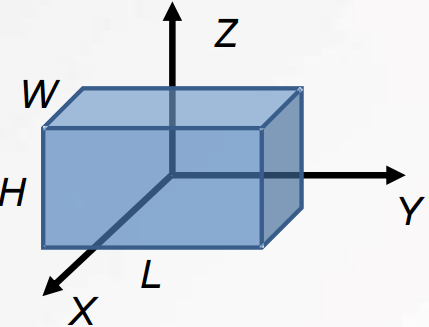
\includegraphics[width=.2\textwidth]{6.1}} \quad
\subfloat[位于一角]{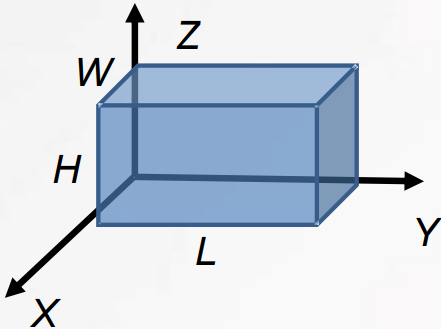
\includegraphics[width=.2\textwidth]{6.2}}
\caption[惯性张量例题]{惯性张量例题}
\end{figure}
\begin{enumerate}
\item 位于中心:
\begin{align*}
I_{xx} &= \int_{-\frac{H}{2}}^{\frac{H}{2}} \int_{-\frac{L}{2}}^{\frac{L}{2}} \int_{-\frac{W}{2}}^{\frac{W}{2}} (y^2 + z^2)\rho dxdydz = \frac{H^2 + L^2}{12} LWH\rho = \frac{m}{12}(H^2 + L^2) \\
I_{xy} &= \int_{-\frac{H}{2}}^{\frac{H}{2}} \int_{-\frac{L}{2}}^{\frac{L}{2}} \int_{-\frac{W}{2}}^{\frac{W}{2}} (xy)\rho dxdydz = 0
\end{align*}
\item 位于一角,利用平行轴定理:
\begin{align*}
I_{Axx} &= I_{Cxx} + m(y_C^2 + z_C^2) = \frac{m}{12}(H^2 + L^2) + \frac{m}{4}(H^2 + L^2) = \frac{m}{3}(H^2 + L^2) \\
I_{Axy} &= I_{Cxy} + m x_C y_C = \frac{m}{4}WL
\end{align*}
\end{enumerate}
}
%------------------------------------------------
\subsection[牛顿-欧拉动力学方程]{牛顿-欧拉动力学方程}
%------------------------------------------------
\subsubsection[推导]{推导}
%------------------------------------------------
\paragraph{动力学受力分析}\label{sec:fn2}
\textcolor{red}{与静力学受力分析对比}\ref{sec:fn1}

\begin{figure}[H]
\centering 
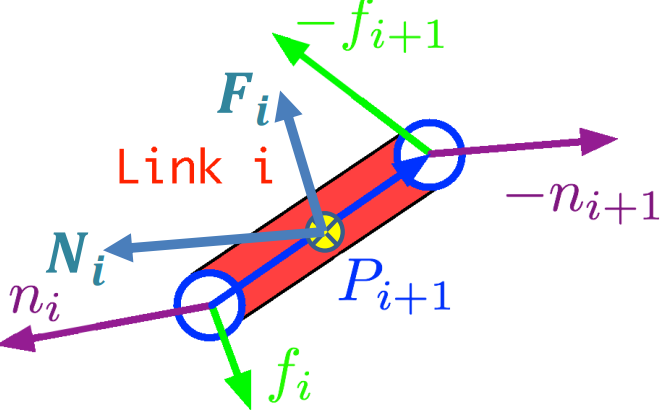
\includegraphics[width=0.3\textwidth]{force2} 
\caption[动力学受力分析]{动力学受力分析}
\end{figure}

$$
\begin{cases}
f_i &= f_{i + 1} \textcolor{red}{+ F_i} \\
n_i &= n_{i + 1} + P_{i + 1} \times f_{i + 1} \textcolor{red}{+ P_{C_i} \times F_i + N_i} \\
\end{cases}
$$
%------------------------------------------------
\paragraph{牛顿-欧拉动力学方程}
\begin{itemize}
\item 牛顿方程:$ F = \dot{Q} = ma $。
\item 欧拉方程:$ N = \dot{L} = \frac{d}{dt}(\vec{m}||\omega||) = \dot{\vec{m}}||\omega|| + \vec{m}||\dot{\omega}|| = \omega \times \vec{m}||\omega|| + I\dot{\omega} = \omega \times I\omega + I\dot{\omega} $。
\end{itemize}
%------------------------------------------------
\paragraph{关节分析(外推)}
\begin{figure}[H]
\centering
\subfloat[速度与加速度]{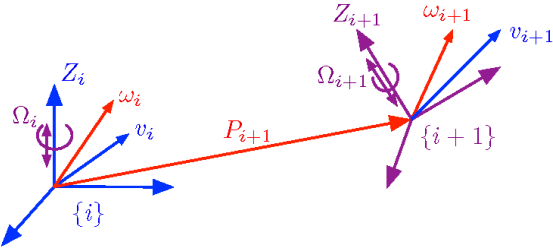
\includegraphics[width=.4\textwidth]{Velocity propagation}} \quad
\subfloat[受力]{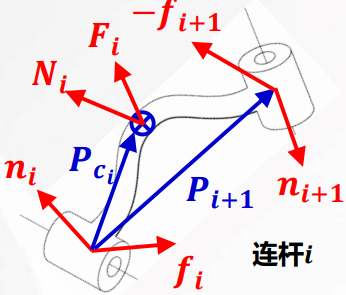
\includegraphics[width=.25\textwidth]{Force Analysis}}
\caption[关节分析]{关节分析}
\end{figure}

\begin{itemize}
\item 速度:
\begin{align*}
v_{i + 1} &=  v_i + \omega_i \times P_{i + 1} + \dot{d}_{i + 1} \cdot Z_{i + 1} \\
\omega_{i + 1} &=  \omega_i + \dot{\theta}_{i + 1} \cdot Z_{i + 1}
\end{align*}
\item 加速度:(\textcolor{blue}{平移关节})
\begin{align*}
\dot{v}_{i + 1} &=  \dot{v}_i +  \dot{\omega}_i \times P_{i + 1} + \textcolor{blue}{\ddot{d}_{i + 1} \cdot Z_{i + 1}} + \underbrace{\omega_i \times \overset{\omega_i \times P_{i + 1}}{\overbrace{\dot{P_{i + 1}}}}}_{\text{离心力}} + \underbrace{\textcolor{blue}{2\dot{d}_{i + 1} \omega_i \times Z_{i + 1}}}_{\text{科里奥利力}} \\
\dot{\omega}_{i + 1} &=  \dot{\omega}_i + \ddot{\theta}_{i + 1} \cdot Z_{i + 1} + \dot{\theta}_{i + 1} \cdot \underbrace{\dot{Z_{i + 1}}}_{\omega_i \times Z_{i + 1}}
\end{align*}
\item 质心处速度:($ P_{C_{i + 1}} $为到质心的向量)
\begin{align*}
v_{C_{i + 1}} &= v_{i + 1} + \omega_{i + 1} \times P_{C_{i + 1}} \\
\omega_{C_{i + 1}} &= \omega_{i + 1}
\end{align*}
\item 质心处速度:
\begin{align*}
\dot{v}_{C_{i + 1}} &= \dot{v}_{i + 1} + \dot{\omega}_{i + 1} \times P_{C_{i + 1}} + \omega_{i + 1} \times (\omega_{i + 1} \times P_{C_{i + 1}}) \\
\dot{\omega}_{C_{i + 1}} &= \dot{\omega}_{i + 1}
\end{align*}
\item 连杆惯性力(矩):
\begin{align*}
F_{i + 1} &= m_{i + 1} \dot{v}_{C_{i + 1}} \\
N_{i + 1} &= I_{C_{i + 1}} \dot{\omega}_{i + 1} + \omega_{i + 1} \times I_{C_{i + 1}} \omega_{i + 1}
\end{align*}
\item 质心处受力分析:
\begin{align*}
F_i &= f_i - f_{i + 1} = m_i \dot{v}_{C_i} \\
N_i &= n_i - n_{i + 1} + (-P_{C_i}) \times f_i + (P_{i + 1} - P_{C_i}) \times (-f_{i + 1})
\end{align*}
\end{itemize}
%------------------------------------------------
\subsubsection[总结]{总结\tip{牛顿-欧拉动力学方程建模}}
外推速度、加速度、受力(连杆->质心),内推力矩。

\begin{figure}[H]
\centering 
\includegraphics[width=0.5\textwidth]{Newton Euler} 
\caption[建模过程]{建模过程}
\end{figure}

统一坐标系:
\begin{align*}
^{i + 1}v_{i + 1} &= \textcolor{red}{^{i + 1}_iR} \cdot ^iv_i + \textcolor{red}{^{i + 1}_iR} (\textcolor{blue}{^i\omega_i} \times \textcolor{cyan}{^iP_{i + 1}}) + \textcolor{violet}{\dot{d}_{i + 1}} \cdot \textcolor{magenta}{^{i + 1}Z_{i + 1}} \\
\textcolor{orange}{^{i + 1}\omega_{i + 1}} &= \textcolor{red}{^{i + 1}_iR} \cdot \textcolor{blue}{^i\omega_i} + \textcolor{teal}{\dot{\theta}_{i + 1}} \cdot \textcolor{magenta}{^{i + 1}Z_{i + 1}} \\
\textcolor{pink}{^{i + 1}\dot{v}_{i + 1}} &= \textcolor{red}{^{i + 1}_iR} \cdot [^i\dot{v}_i + ^i\dot{\omega}_i \times \textcolor{cyan}{^iP_{i + 1}} + \textcolor{blue}{^i\omega_i} \times (\textcolor{blue}{^i\omega_i} \times \textcolor{cyan}{^iP_{i + 1}})] + \ddot{d}_{i + 1} \cdot \textcolor{magenta}{^{i + 1}Z_{i + 1}} + 2\textcolor{violet}{\dot{d}_{i + 1}} \cdot ^{i + 1}\omega_i \times \textcolor{magenta}{^{i + 1}Z_{i + 1}} \\
\textcolor{purple}{^{i + 1}\dot{\omega}_{i + 1}} &= \textcolor{red}{^{i + 1}_iR} \cdot ^i\dot{\omega}_i + \ddot{\theta}_{i + 1} \cdot \textcolor{magenta}{^{i + 1}Z_{i + 1}} + \textcolor{teal}{\dot{\theta}_{i + 1}} \cdot (\textcolor{red}{^{i + 1}_iR} \cdot \textcolor{blue}{^i\omega_i} \times \textcolor{magenta}{^{i + 1}Z_{i + 1}}) \\
\textcolor{brown}{^{i + 1}\dot{v}_{C_{i + 1}}} &= \textcolor{pink}{^{i + 1}\dot{v}_{i + 1}} + \textcolor{purple}{^{i + 1}\dot{\omega}_{i + 1}} \times \textcolor{lime}{^{i + 1}P_{C_{i + 1}}} + \textcolor{orange}{^{i + 1}\omega_{i + 1}} \times (\textcolor{orange}{^{i + 1}\omega_{i + 1}} \times \textcolor{lime}{^{i + 1}P_{C_{i + 1}}}) \\
^{i + 1}F_{i + 1} &= m_{i + 1} \cdot \textcolor{brown}{^{i + 1}\dot{v}_{C_{i + 1}}} \\
^{i + 1}N_{i + 1} &= \textcolor{yellow}{^{i + 1}I_{C_{i + 1}}} \cdot \textcolor{purple}{^{i + 1}\dot{\omega}_{i + 1}} + \textcolor{orange}{^{i + 1}\omega_{i + 1}} \times \textcolor{yellow}{^{i + 1}I_{C_{i + 1}}} \cdot \textcolor{orange}{^{i + 1}\omega_{i + 1}} \\
\textcolor{gray}{^if_i} &= ^iF_i + \textcolor{green}{^i_{i + 1}R} \cdot ^{i + 1}f_{i + 1} \\
\textcolor{olive}{^in_i} &= ^iN_i + \textcolor{green}{^i_{i + 1}R} \cdot ^{i + 1}n_{i + 1} + ^iP_{C_i} \times ^iF_i + \textcolor{cyan}{^iP_{i + 1}} \times \textcolor{green}{^i_{i + 1}R} \cdot ^{i + 1}f_{i + 1} \\
\tau_i &= 
\begin{cases} 
\textcolor{olive}{^in_i} \cdot Z_i & \text{旋转关节} \\ 
\textcolor{gray}{^if_i} \cdot Z_i & \text{平移关节} 
\end{cases}
\end{align*}

基坐标系固定时的初始值(表征重力):
$$ ^0\omega_0 = 0, ^0v_0 = 0, ^0\dot{v}_0 = g $$
%------------------------------------------------
\paragraph{例题}~\\
{\footnotesize
\begin{minipage}{0.35\textwidth}
\begin{figure}[H]
\centering 
\includegraphics[width=0.85\textwidth]{7} 
\caption[牛顿-欧拉动力学方程例题]{牛顿-欧拉动力学方程例题}
\end{figure}
\end{minipage}
\hfill
\begin{minipage}{0.6\textwidth}
RP平面机器人的连杆质量分别为$ m_1,m_2 $,连杆质心距关节$ 1 $距离分别为$ l_1,d_2 $,连杆质心处惯性张量分别为:
$$
{^{C_1}}I_1 = \begin{bmatrix} I_{xx1} & 0 & 0 \\ 0 & I_{yy1} & 0 \\ 0 & 0 & I_{zz1} \end{bmatrix},
{^{C_2}}I_2 = \begin{bmatrix}  I_{xx2} & 0 & 0 \\ 0 & I_{yy2} & 0 \\ 0 & 0 & I_{zz2} \end{bmatrix}
$$
统一到$ 1 $坐标系下:$ y_1 $与$ z_2 $重合:
$$ ^1P_2 = \begin{bmatrix} 0 & q_2 & 0 \end{bmatrix}^T, ^1P_{C_2} = \begin{bmatrix} 0 & d_2 & 0 \end{bmatrix}^T $$
\end{minipage}

\begin{enumerate}
\item 初始条件: $ ^0\omega_0 = 0, ^0v_0 = 0, ^0\dot{\omega}_0 = 0, ^0\dot{v}_0 = \begin{bmatrix} 0 & g & 0 \end{bmatrix}^T, f_3 = 0, n_3 = 0 $。
\item 关节$ 1 $运动学:
\begin{align*}
^1\omega_1 &= \dot{q}_1 \cdot ^1Z_1 = \begin{bmatrix} 0 & 0 & \dot{q}_1 \end{bmatrix}^T \\
^1\dot{\omega}_1 &= \ddot{q}_1 \cdot ^1Z_1 = \begin{bmatrix} 0 & 0 & \ddot{q}_1 \end{bmatrix}^T \\
^1\dot{v}_1 &= ^1_0R_z(\theta_1) \cdot ^0\dot{v}_0 = \begin{bmatrix} gs1 & gc1 & 0 \end{bmatrix}^T \\
^1\dot{v}_{C_1} &= ^1\dot{v}_1 + ^1\dot{\omega}_1 \times ^1P_{C_1} + ^1\omega_1 \times (^1\omega_1 \times ^1P_{C_1}) = \begin{bmatrix} -l_1\dot{q}_1^2 + gs1 & -l_1\ddot{q}_1 + gc1 & 0 \end{bmatrix}^T
\end{align*}
\item 关节$ 1 $力:
\begin{align*}
^1F_1 &= m_1 \cdot ^1\dot{v}_{C_1} \\
^1N_1 &= ^{C_1}I_1 \times ^1\dot{\omega}_1 + ^1\omega_1 \times ^{C_1}I_1 \cdot ^1\omega_1 = \begin{bmatrix} 0 & 0 & \ddot{q}_1 I_{zz1} \end{bmatrix}^T
\end{align*}
\item 关节$ 2 $运动学:
\begin{align*}
^1\omega_2 &= ^1\omega_1 = \begin{bmatrix} 0 & 0 & \dot{q}_1 \end{bmatrix}^T \\
^1\dot{\omega}_2 &= ^1\dot{\omega}_1 = \begin{bmatrix} 0 & 0 & \ddot{q}_1 \end{bmatrix}^T \\
^1\dot{v}_2 &= ^1\dot{v}_1 + ^1\dot{\omega}_1 \times ^1P_2 + ^1\omega_1 \times (^1\omega_1 \times ^1P_2) + \ddot{q}_2 \cdot ^1Z_2 + 2\dot{q}_2 \cdot ^1\omega_1 \times ^1Z_2 \\
&= \begin{bmatrix} -\ddot{q}_1q_2 - 2\dot{q}_1\dot{q}_2 + gs1 & -\dot{q}_1^2q_2 + {\ddot{q}_2}^2 + gc1 & 0 \end{bmatrix}^T \\
^1\dot{v}_{C_2} &= ^1\dot{v}_2 + ^1\dot{\omega}_2 \times ^1P_{C_2} + ^1\omega_2 \times (^1\omega_2 \times ^1P_{C_2}) \\
&= \begin{bmatrix} -2\dot{q}_1\dot{q}_2 + gs1 - \ddot{q}_1(d_2 + q_2) & \ddot{q}_2 + gc1 - \dot{q}_1^2(d_2 + q_2) & 0 \end{bmatrix}^T
\end{align*}
\item 关节$ 2 $力:
\begin{align*}
^1F_2 &= m_2 \cdot ^1\dot{v}_{C_2} = \begin{bmatrix} -2m_2\dot{q}_1\dot{q}_2 + m_2gs1 - m_2\dot{q}_1^2(d_2 + q_2) & m_2\ddot{q}_2 + m_2gc1 - m_2\dot{q}_1^2(d_2 + q_2) & 0 \end{bmatrix}^T \\
^1N_2 &= ^{C_2}I_2 \times ^1\dot{\omega}_2 + ^1\omega_2 \times ^{C_2}I_2 \cdot ^1\omega_2 = \begin{bmatrix} 0 & 0 & \ddot{q}_1 I_{zz2} \end{bmatrix}^T
\end{align*}
\item 关节$ 2 $力矩:
\begin{align*}
^1f_2 &= ^1F_2 \\
^1n_2 &= ^1N_2 + ^1P_{C_2} \times ^1F_2 = \begin{bmatrix} 0 & 0 & \ddot{q}_1 I_{zz2} + 2m_2d_2\dot{q}_1\dot{q}_2 - m_2d_2gs1 + m_2d_2\ddot{q}_1(d_2 + q_2) \end{bmatrix}^T
\end{align*}
\item 关节$ 1 $力矩:
\begin{align*}
^1f_1 &= ^1F_1 + ^1f_2 \\
^1n_1 &= ^1N_1 + ^1n_2 + ^1P_{C_1} \times ^1F_1 + ^1P_2 \times ^1f_2 \\
&= \begin{bmatrix} \star & \star & \ddot{q}_1[I_{zz2} + I_{zz1} + m_1l_1^2 + m_2(d_2 + q_2)^2] + 2m_2\dot{q}_1\dot{q}_2(d_2 + q_2) - [m_1l_1 + m_2(d_2 + q_2)]gs1 \end{bmatrix}^T
\end{align*}
\item 力矩:
\begin{align*}
\tau_2 &= ^1f_2 \cdot ^1Z_2 = m_2\ddot{q}_2 + m_2gc1 - m_2\dot{q}_1^2(d_2 + q_2) \\
\tau_1 &= ^1n_1 \cdot ^1Z_1 = \ddot{q}_1[I_{zz2} + I_{zz1} + m_1l_1^2 + m_2(d_2 + q_2)^2] + 2m_2\dot{q}_1\dot{q}_2(d_2 + q_2) - [m_1l_1 + m_2(d_2 + q_2)]gs1
\end{align*}
\item 标准形式:
\begin{align*}
\Gamma = \begin{bmatrix} \tau_1 & \tau_2 \end{bmatrix}^T &= \begin{bmatrix} \ddot{q}_1[I_{zz2} + I_{zz1} + m_1l_1^2 + m_2(d_2 + q_2)^2] & 0 \\ 0 & m_2 \end{bmatrix} \ddot{q} \\
&+ \begin{bmatrix} 2m_2(d_2 + q_2) & 0 \\ 0 & m_2(d_2 + q_2) \end{bmatrix} \begin{bmatrix} \dot{q}_1\dot{q}_2 \\ \dot{q}_1^2 \end{bmatrix} + \begin{bmatrix} - [m_1l_1 + m_2(d_2 + q_2)]s1 \\ m_2c1 \end{bmatrix} g 
\end{align*}
\end{enumerate}
}
%------------------------------------------------
\subsection[拉格朗日动力学算法]{拉格朗日动力学算法\tip{拉格朗日动力学算法}}
%------------------------------------------------
\subsubsection[拉格朗日动力学方程]{拉格朗日动力学方程}
%------------------------------------------------
\paragraph{系统能量分析}
\begin{itemize}
\item 势能$ U(q, t) $:
\begin{itemize}
\item 与速度:无关,$ \textcolor{red}{\frac{\partial U}{\partial \dot{q}} = 0} $。
\item 与位移:克服的弹力或重力,$ \textcolor{green}{\frac{\partial U}{\partial q} = G(q)} $。
\end{itemize}
\item 动能$ K(q, \dot{q}, t) = \frac{1}{2}\dot{q}^T M(q)\dot{q} $(其中$ q $为$ v/\omega $,$ M $为$ m/I $):瞬时性,正标量
\begin{itemize}
\item 与速度:(角)动量,$ \textcolor{orange}{\frac{\partial K}{\partial \dot{q}} = Q(q, \dot{q})} $,其变化率为惯性力$ \textcolor{orange}{F = \frac{d Q(q, \dot{q})}{d t}} $。
\item 与位移(构型变化):内力做功,$ \textcolor{blue}{\frac{\partial K}{\partial q} = \frac{\partial M(q)}{\partial q}}  $。
\end{itemize}
\end{itemize}
%------------------------------------------------
\paragraph{拉格朗日动力学方程}
系统输入(广义外力)$ \Gamma $
\begin{align*}
\Gamma &= \underbrace{\textcolor{orange}{\frac{d}{d t}\frac{\partial K}{\partial \dot{q}}} - \textcolor{blue}{\frac{\partial K}{\partial q}}}_{\text{惯性力}M(q)\ddot{q} + V(q,\dot{q})} + \underbrace{\textcolor{green}{\frac{\partial U}{\partial q}}}_{\text{重力}G(q)} \\
&= \frac{d}{d t}\frac{\partial(K - \textcolor{red}{U})}{\partial \dot{q}} - \frac{\partial(K - U)}{\partial q} \\
&= \frac{d}{d t}\frac{\partial L}{\partial \dot{q}} - \frac{\partial L}{\partial q}
\end{align*}

其中,$ L(q, \dot{q}, t) = K(q, \dot{q}, t) - U(q, t) $;$ q,\dot{q} \in R^n $为广义坐标和广义速度,它们相互独立。对于各关节,有:

$$ \tau_i = \frac{d}{d t}\frac{\partial L(q, \dot{q}, t)}{\partial \dot{q}_i} - \frac{\partial L(q, \dot{q}, t)}{\partial q_i} \quad i = 1, 2, \cdots, N $$
%------------------------------------------------
\paragraph{推导}
\begin{align*}
\frac{\partial}{\partial\dot{q}}K(q, \dot{q}) = M(q)\dot{q} \Rightarrow \frac{d}{d t}(\frac{\partial}{\partial\dot{q}}K(q, \dot{q})) = M(q)\ddot{q} + \dot{M}(q)\dot{q} \\
\frac{\partial}{\partial q}K(q,\dot{q}) = \frac{\partial}{\partial q}[\frac{1}{2}\dot{q}^T M(q)\dot{q}] = \frac{1}{2} \begin{bmatrix} \dot{q}^T\frac{\partial M(q)}{\partial q_1}\dot{q} \\ \vdots \\ \dot{q}^T\frac{\partial M(q)}{\partial q_N}\dot{q} \end{bmatrix}
\end{align*}

所以:
$$ \frac{d}{dt}\frac{\partial K(q,\dot{q})}{\partial\dot{q}} - \frac{\partial K(q,\dot{q})}{\partial q} = \underbrace{M(q)\ddot{q}}_{\text{惯性力}} + \underbrace{\dot{M}(q)\dot{q} - \frac{1}{2}\begin{bmatrix} \dot{q}^T\frac{\partial M(q)}{\partial q_1}\dot{q} \\ \vdots \\ \dot{q}^T\frac{\partial M(q)}{\partial q_N}\dot{q} \end{bmatrix}}_{\text{科里奥利力}} $$

需求解惯性阵$ M(q) $,可通过求解系统动能$ K(q, \dot{q}) $获得。
%------------------------------------------------
\subsubsection[系统动能]{系统动能}
%------------------------------------------------
\paragraph{多体动力学}~\\

连杆$ i $动能$ K_i(q, \dot{q}) = \frac{1}{2}v_{C_i}^T mv_{C_i} + \frac{1}{2}\omega_{C_i}^T I_C\omega_{C_i} $,

故机器人系统总动能:
$$ K(q, \dot{q}) = \sum_{i = 1}^{n} K_i = \sum_{i=1}^{n} (\frac{1}{2}v_{C_i}^T mv_{C_i} + \frac{1}{2}\omega_{C_i}^T I_C\omega_{C_i}) $$
%------------------------------------------------
\paragraph{惯性阵$ M(q) $求取}\label{sec:bingxing_back2}
\begin{align*}
K(q, \dot{q}) = \frac{1}{2}\dot{q}^T \textcolor{red}{M(q)} \dot{q} &\equiv \sum_{i=1}^{n}(\frac{1}{2}v_{C_i}^T m_i v_{C_i} + \frac{1}{2}\omega_{C_i}^T I_{C_i}\omega_{C_i}) \\
&= \sum_{i = 1}^{n}(\frac{1}{2}\dot{q}^T J_{v_{C_i}}^T m_i J_{v_{C_i}} \dot{q} + \frac{1}{2}\dot{q}^T J_{\omega_{C_i}}^T I_{C_i} J_{\omega_{C_i}} \dot{q}) \\
&= \frac{1}{2}\dot{q}^T \textcolor{red}{\sum_{i = 1}^{n}[J_{v_{C_i}}^T m_i J_{v_{C_i}} + J_{\omega_{C_i}}^T I_{C_i} J_{\omega_{C_i}}]} \dot{q}
\end{align*}

其中$ J_{v_{C_i}},J_{\omega_{C_i}} $为连杆$ i $质心处的雅可比,可由雅可比转化(见\ref{sec:bingxing})推得,未涉及到的变化(即关节$ i $之后的变化)的位置为$ 0 $。
%----------------------------------------------------------------------------------------
\section{轨迹规划}
%------------------------------------------------
\section{机器人控制}
%----------------------------------------------------------------------------------------
\end{document}